\chapter[Absorbing Sets of Array-based LDPC Codes]{Absorbing Sets of Array-based LDPC
Codes}\label{arrayabs}

In this Chapter we provide a detailed analysis of the  minimal
absorbing sets and minimal fully absorbing sets of the high rate
array-based LDPC codes.


%\section{Background}\label{back}
\section{Array-based LDPC Code Construction}
% no \PARstart
%This demo file is intended to serve as a ``starter file"
%for IEEE conference papers produced under \LaTeX\ using IEEEtran.cls version
%1.6b and later.

% May all your publication endeavors be successful.

%\hfill mds

%\hfill November 18, 2002

Array based LDPC codes \cite{fan} are regular LDPC codes
parameterized by a pair of integers $(\gamma, p)$, such that
$\gamma \leq p$, $p$ is an odd prime, with a parity check matrix
$H_{p,\gamma}$ given by
\begin{equation}\label{eq:1}
H_{p,\gamma}=\left[\begin{array}{ccccc}
I & I & I & \ldots & I\\
I & \sigma & \sigma^2 & \ldots &\sigma^{p-1}\\
I & \sigma^2 & \sigma^4 & \ldots &\sigma^{2(p-1)}\\
\vdots & \vdots & \vdots & \ldots & \vdots \\
I & \sigma^{\gamma-1} & \sigma^{(\gamma-1)2} & \ldots &\sigma^{(\gamma-1)(p-1)}\\
\end{array}
\right]
\end{equation}\normalsize
where $\sigma$ denotes a $p \times p$ permutation matrix of the
form \small
\begin{equation}
\sigma=\left[\begin{array}{ccccc}
0 & 0 & \ldots & 0 & 1\\
1 & 0 & \ldots & 0 & 0\\
0 & 1 & \ldots & 0 & 0\\
\vdots & \vdots & \ldots & \vdots & \vdots\\
0 & 0 & \ldots & 1 & 0\\
\end{array}
\right].
\end{equation}
\normalsize We use $C_{p,\gamma}$ to denote the binary linear code
with parity check matrix of the form \eqref{eq:1}. The rate of
this code is $R=1-\frac{\gamma p-\gamma+1}{p^2}$,
\cite{mittel:02}.

As first demonstrated by Fan \cite{fan}, array-based LDPC codes
have very good performance. They have been proposed for a number
of applications, including digital subscriber lines \cite{ibm:02}
and magnetic recording  \cite{vasic:05}.




\comment{In our earlier experimental work \cite{zhang06}, we have
observed that certain structures in the Tanner graph of the parity
check matrix of the code are the limiting factor in the iterative
decoding of several structured LDPC codes, including array-based
codes. Motivated by the empirical findings, we formally defined
these configurations, which we call \emph{absorbing sets}.Here we
study them in detail for array-based LDPC codes $C_{p,\gamma}$ for
$\gamma=2,3,4$, for the standard parity check matrix
$H_{p,\gamma}$.}

%We now formally introduce the notion of an absorbing set useful in
%studying the limiting behavior of the message passing algorithm in
%the very low BER region.

\comment{\subsection{Absorbing Sets} Let $G=(V,F,E)$ be a
bipartite graph with the vertex set $V \cup F$, where $V$ and $F$
are disjoint, and with the edge set $E$, such that there exists an
edge $e(i,j) \in E$ iff $i\in V$ and $j\in F$. One can associate a
bipartite graph $G_H=(V,F,E)$ with a parity check matrix $H$, such
that the set $V$ corresponds to the columns of $H$, the set $F$
corresponds to the rows of $H$, and $E=\{ e(i,j)| H(j,i)=1\}$.
Such a graph $G_H$ is commonly referred to as the Tanner graph of
the parity check matrix $H$ of a code, \cite{forney}. Elements of
$V$ are called ``bit nodes'' and elements of $F$ are called
``check nodes''. The Tanner graph associated with $H_{p,\gamma}$
does not have any cycles of length 4, and thus the girth is at
least 6 \cite{fan}. For the subset $D$ of $V$ we let $N_D$ denote
the set of check nodes neighboring the elements of $D$. For a
subset $D$ of $V$, let $\mathcal{E}(D)$ (resp. $\mathcal{O}(D)$)
be the set of neighboring vertices of $D$ in $F$ in the graph $G$
with even (resp. odd) degree with respect to $D$. With this set-up
we have the following.
\begin{definition}  Given an integer pair $(a,b)$, an $(a,b)$ \emph{absorbing
set} is a subset $D \subseteq V$ of size $a$, with
$\mathcal{O}(D)$ of size $b$ and with the property that each
element of $D$ has strictly fewer neighbors in $\mathcal{O}(D)$
than in $F\backslash \mathcal{O}(D)$. We say that an $(a,b)$
absorbing set $D$ is an $(a,b)$ \emph{fully absorbing set}, if in
addition, all bit nodes in $V\backslash D$ have strictly more
neighbors in $F\backslash \mathcal{O}(D)$ than in
$\mathcal{O}(D)$.\end{definition} An example of an $(a,b)$
absorbing set with $(a,b) = (4,4)$ is given in Figure \ref{abs44},
where full circles constitute the set $D$, full squares constitute
the set $\mathcal{O}(D)$, white squares constitute the set
$\mathcal{E}(D)$, $E(D,\mathcal{O}(D))$ is given by solid lines,
and $E(D,\mathcal{E}(D)$ is given by dashed lines. Observe that
each element in $D$ has more even-degree than odd-degree
neighbors. All check nodes not in the picture are denoted by white
squares. For this set to be a fully absorbing set, every bit node
not in the figure should also have strictly more empty squares
than full squares as neighbors.
%In the remainder, when we say that the $(a,b)$ absorbing sets do
%(do not) exist for a particular code, we will implicitly refer to
%the existence (non existence) of $(a,b)$ absorbing sets in the
%Tanner graph associated with the given code.
Note that $D \subseteq V$ is a fully absorbing set if and only if
for all $v \in D$, $wt$$(Hx_{D \Delta v})$ $>$ $wt$$(Hx_D)=b$,
where $D \Delta v$ denotes the symmetric difference between $D$
and $\{v\}$, $wt(y)$ is the Hamming weight of a binary string $y$,
and $x_D$ is a binary string with support $D$.
\begin{figure}
\center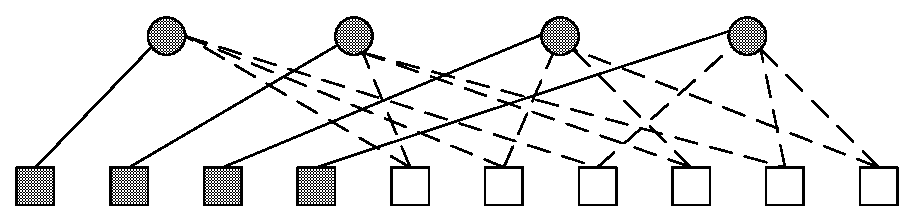
\includegraphics[width=3.0in,height=0.9in]{Drawing11.eps}
\caption{An example of a (4,4) absorbing set} \label{abs44}
\end{figure}}


\comment{Moreover, an $(a,b)$ absorbing set can also be
interpreted as follows. For an integer $a$ let $c_a:=c+x_a$, where
$c$ is an arbitrary codeword in the code with the parity check
matrix $H$, and where $x_a$ is a binary vector with non zero
entries in precisely $a$ positions. Let $s_a=Hc_a$, and let $b$ be
the weight of $s_a$. If the weight of $s_a$ strictly increases
when the support of $x_a$ is decreased, the vertex induced
subgraph in $G_H$ induced by the support of $x_a$ and the support
of $s_a$ represents an $(a,b)$ absorbing set.}



\comment{We have introduced the notion of absorbing sets to
qualitatively describe the convergent non-codeword state of the
message passing algorithms, when the transmission channel is
additive white Gaussian noise (AWGN). For the special case of a
bit flipping algorithm, the configuration described as a fully
absorbing set is stable, since each bit node receives strictly
more messages from the neighboring checks that reinforce its value
than messages that suggest the opposite bit value. In particular,
a fully absorbing set can be viewed as a near codeword as defined
in \cite{mackay}, though the reverse is not true, since a near
codeword does not necessarily describe a stable configuration.
Although stopping sets \cite{di_stop} also describe stable
configurations, they are defined in the context of a binary
erasure channel, and cannot be directly applied to an AWGN
channel. The trapping sets were introduced in \cite{richardson}
operationally, as a function of the decoding algorithm. Also they
do not explicitly capture the convergent behavior of a decoder
since they refer to the union of all bits that are not eventually
correct, and thus permit a situation in which the decoder
oscillates among a finite number of states.}
\section{Theoretical Results}\label{theo1}

Our goal is to describe minimal absorbing sets and minimal fully
absorbing sets $(a,b)$ of the Tanner graph of the parity check
matrix $H_{p,\gamma}$, for $\gamma =2,3,4$, where the minimality
refers to the smallest possible $a$, and where $b$ is the smallest
possible for the given $a$.

We use the following notation throughout the paper. Recall that
$H_{p,\gamma}$ is a $\gamma p \times p^2$ matrix of 0's and 1's. It
is convenient to view $H_{p,\gamma}$ as a two-dimensional array of
component $p \times p$ submatrices with the rows $i$ in the range $0
\leq i \leq \gamma-1$ (also referred to as row groups) and the
columns $j$ in the range $0 \leq j \leq p-1$ (also referred to as
column groups). Each column of $H_{p,\gamma}$ is uniquely described
by a pair $(j,k)$ where $j$ denotes the column index of the
submatrix this column belongs to, and $k$, $0 \leq k \leq p-1$
denotes the index of this column within the submatrix.

\begin{figure}
\center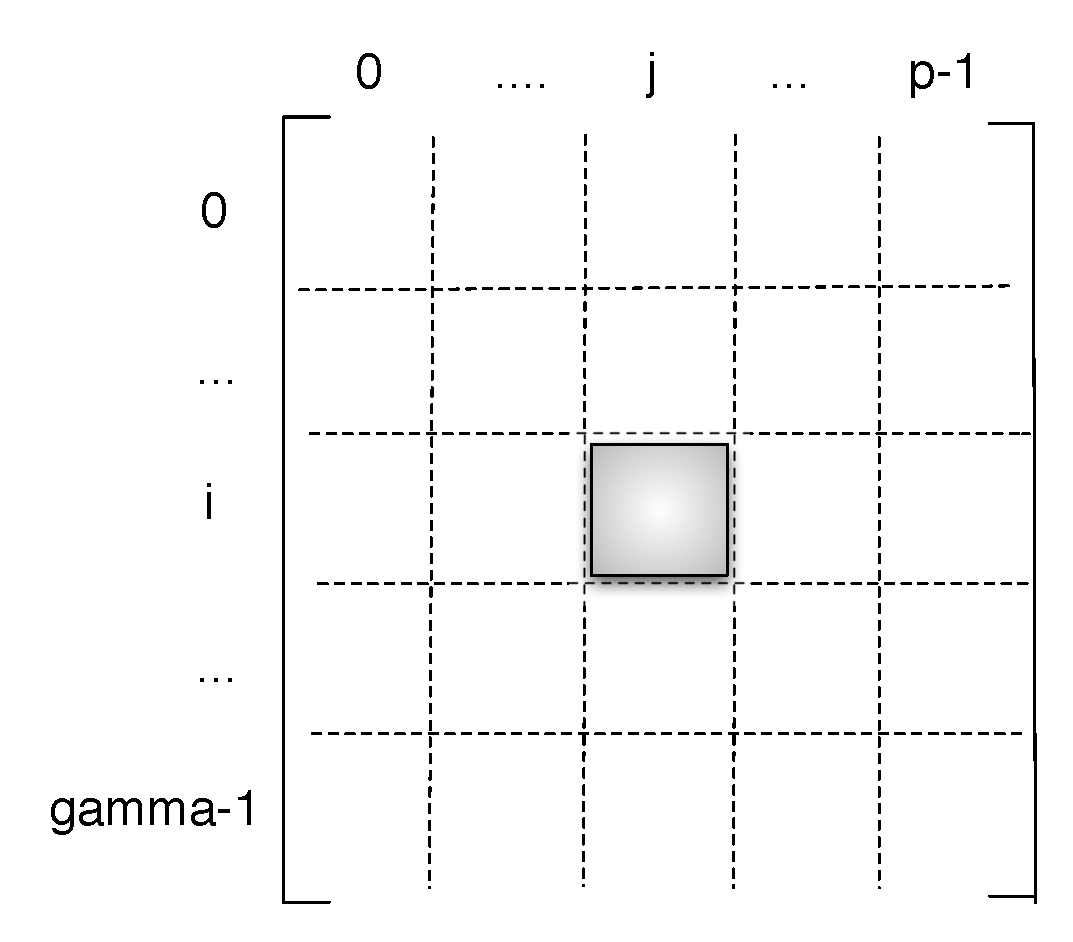
\includegraphics[width=2.8in,height=1.8in]{matrix1.eps}
\\
\hspace{0.65in}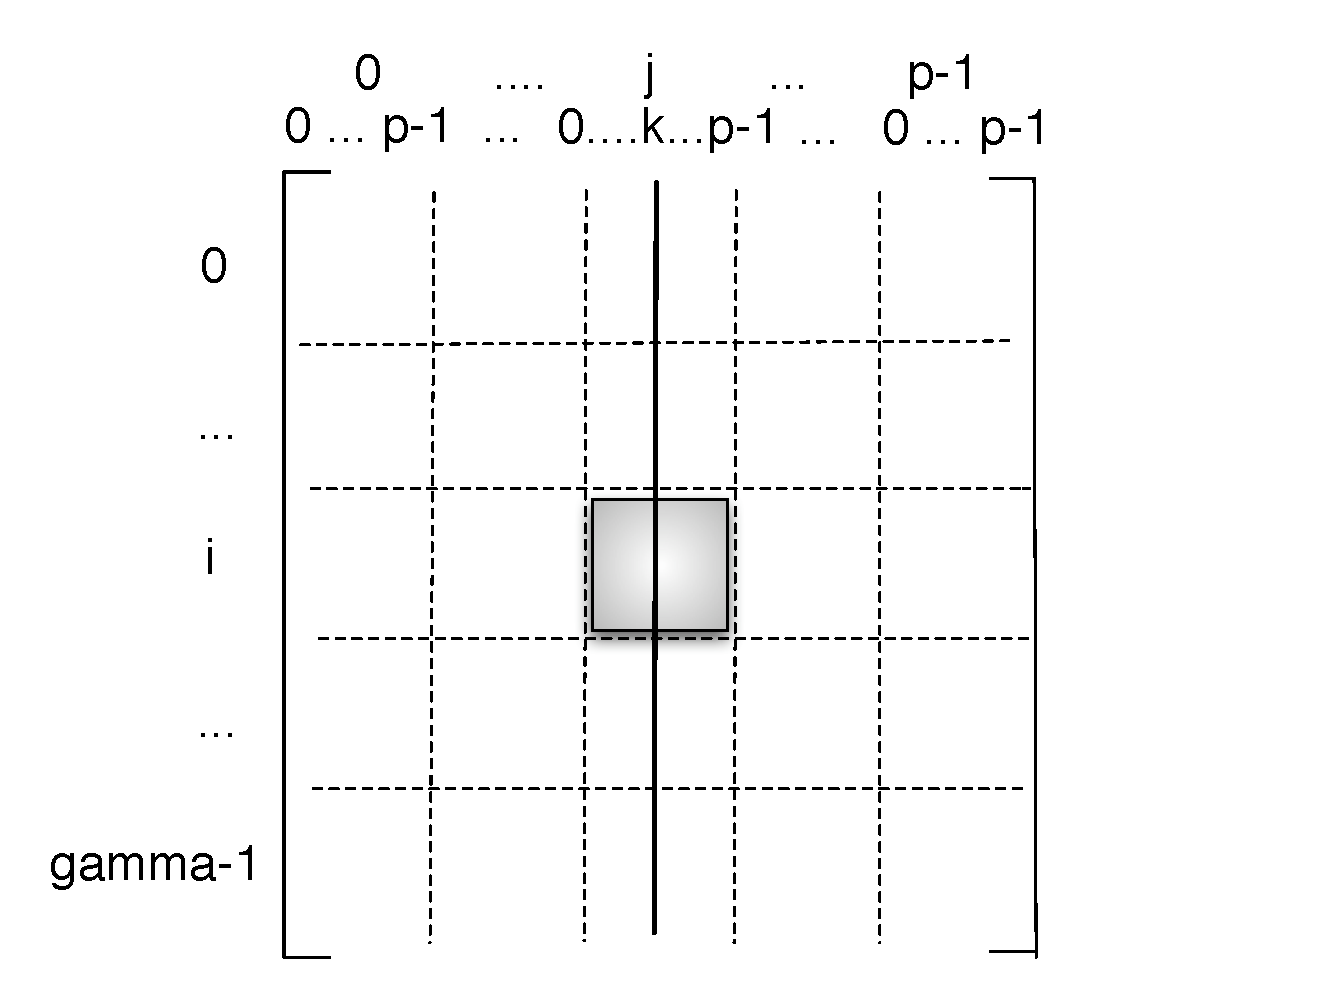
\includegraphics[width=3.4in,height=2.0in]{matrix2.eps}
\caption{Illustration of the notation (a) Row and column groups in
$H_{p,\gamma}$(b) $(j,k)$ column label. Shaded area corresponds to
the submatrix $\sigma^{ij}$} \label{fig62}
\end{figure}
%, corresponding to the column-wise index in $H_{p,\gamma}$, and
%denoted the column group $j$. Likewise let $i$ in the interval $0
%\leq i \leq \gamma-1$ be the row-wise index in $H_{p,\gamma}$ and
%denoted the row group (or the label) $i$.

Let $G_{p,\gamma}$ be the Tanner graph associated with
$H_{p,\gamma}$, such bit nodes and check nodes in $G_{p,\gamma}$
represent columns and rows in $H_{p,\gamma}$, respectively. In
$G_{p,\gamma}$ bit nodes have degree $\gamma$ and check nodes have
degree $p$. There is a total of $p^2$ bit nodes and $\gamma p$ check
nodes. Each bit node in $G_{p,\gamma}$ receives the unique label
$(j,k)$ that describes the corresponding column of $H_{p,\gamma}$.
Each check node in $G_{p,\gamma}$ receives a label $i$ if
 the corresponding row of $H_{p,\gamma}$ belongs to the row group
$i$. Multiple bit nodes can have the same $j$ or $k$ label, but not
both. Multiple check nodes can have the same $i$ label.

We note that the structure of the parity check matrix imposes the
following conditions on the neighboring bit nodes and check nodes:

\textit{Vertex Consistency:} For a bit node , all its incident check
nodes, labelled $i_{s_1}$ through $i_{s_\gamma}$ must have distinct
labels, i.e. these check nodes are in distinct row groups.

\textit{Edge Consistency:} All bit nodes, say $(j_{1},k_{1})$
through $(j_{p},k_{p})$, participating in the same check node must
have distinct $j_\ell$ values, i.e. they are all in distinct
column groups.

Both conditions follow from the fact that the parity check matrix
$H_{p,\gamma}$ of $C_{p,\gamma}$ consists of a 2-dimensional array
of permutation matrices of equal size.\hfill$\blacksquare$

We begin with elementary lemmas that play a central role throughout
the paper.

\begin{lemma}\textit{Parity check consistency:} Consider the matrices
$\sigma^{ij_1}$ and $\sigma^{ij_2}$ in the same row group of
$H_{p,\gamma}$, \eqref{eq:1}. Suppose the matrix $\sigma^{ij_1}$ has
a non-zero entry in position $(r,k_1)$ (i.e. row $r$ and column
$k_1$) for a given $k_1$. Then, the unique non-zero entry in the row
$r$ of $\sigma^{ij_2}$ is in position $(r,k_2)$ such that
\begin{eqnarray}\label{cong}
k_1+ij_1 \equiv k_2+ij_2 \mod p~.
\end{eqnarray}\end{lemma}

\noindent \textit{Proof:} The congruential constraint
in~\eqref{cong} is derived from the following. Assume that the
columns of $\sigma^{ij}$ are indexed with $0$ through $p-1$. Recall
that $\sigma$ has `1' in the first row in column indexed $p-1$ (last
column), and that each subsequent row has `1' in a position that is
a cyclic shift to the right of the position of `1' in the previous
row. Multiplying $\sigma^{ij}$ with $\sigma$ cyclically shifts the
entries by one position to the left. Thus, $\sigma^{ij_1}$ has `1'
in the first row in column $(p-ij_1) \mod p$, and has `1' in some
row $r$ in the column $k_1 \equiv p-ij_1+r-1 \mod p$.  Likewise,
$\sigma^{ij_2}$ has `1' in this row $r$ in the column indexed $k_2
\equiv p-ij_2+r-1 \mod p$. Equating these expressions in terms of
$r$, the statement in \eqref{cong} follows.\hfill$\blacksquare$

Note that the expression of the type~\eqref{cong} relates the
coordinates of the bit nodes $(j_1,k_1)$ and $(j_2,k_2)$ that both
participate in a check in the row group $i$. We will refer to the
constraint of the type described in~\eqref{cong} as the parity check
consistency constraint.

\begin{lemma}\label{cyclelemma}\textit{Cycle consistency:} Consider a cycle in $G_{p,\gamma}$ of
length $2t$, involving $t$ bit nodes, with labels $(j_1,k_1)$
through $(j_t,k_t)$ and $t$ check nodes, with labels $i_1$ through
$i_t$, such that bit nodes $(j_1,k_1)$ and $(j_2,k_2)$ participate
in the check labelled $i_1$, $(j_2,k_2)$ and $(j_3,k_3)$ participate
in the check labelled $i_2$, and so on, until check labelled $i_t$
in which $(j_t,k_t)$ and $(j_1,k_1)$ participate. Then
\begin{equation}\label{cycles}
i_1(j_2-j_1)+i_2(j_3-j_2)+\dots+i_{t-2}(j_{t-1}-j_{t-2})+i_{t-1}(j_t-j_{t-1})+
i_t(j_1-j_t) \equiv 0 \mod p.
\end{equation}
\end{lemma}
\noindent \textit{Proof:} Using the parity check consistency
constraints as in~\eqref{cong} we then may write
\begin{equation}\begin{array}{cccc}
k_1+i_1j_1 &\equiv&k_2+i_1j_2 & \mod p, \\
k_2+i_2j_2 &\equiv&k_3+i_2j_3 & \mod p, \\
{} & \vdots & {}\\
k_{t-1}+i_{t-1}j_{t-1} &\equiv&k_t+i_{t-1}j_t & \mod p, \\
k_t+i_tj_t &\equiv&k_1+i_tj_1 & \mod p.
\end{array}\end{equation}

Expand $k_1-k_2$ into
$(k_1-k_t)-(k_{t-1}-k_t)-(k_{t-2}-k_{t-1})-\dots-(k_2-k_3)$.
Hence,
\begin{equation}
i_1(j_2-j_1) \equiv
i_t(j_t-j_1)-i_{t-1}(j_t-j_{t-1})-i_{t-2}(j_{t-1}-j_{t-2})-\dots-i_2(j_3-j_2)
\mod p.
\end{equation} By rearranging the terms,~\eqref{cycles} follows.\hfill$\blacksquare$

 The constraint of the type~\eqref{cycles} will subsequently be
referred to as the cycle consistency condition.

We say that the number $Q$ of particular absorbing sets  grows as
$\Theta(n^l)$ if $cn^l \leq Q \leq c'n^l$, for some constants $c$
and $c'$.

Our main results can be summarized as follows: Let $G_{p,\gamma}$
be the Tanner graph associated with the parity check matrix
$H_{p,\gamma}$ of the array-based LDPC code $C_{p,\gamma}$.
\begin{theorem}\label{theo1}\emph{Minimality}

(a) For the $G_{p,2}$ family, all minimal absorbing sets are
minimal fully absorbing sets and are of size $(4,0)$.

(b) For the $G_{p,3}$ family, the minimal absorbing sets are of
size $(3,3)$, and the minimal fully absorbing sets are of size
$(4,2)$.

(c) For the $G_{p,4}$ family, and for $p>19$, all minimal fully
absorbing sets are minimal absorbing sets, and are of size
$(6,4)$.\hfill$\blacksquare$
\end{theorem}
\begin{theorem}\label{theo2}\emph{Scaling}

(a) Suppose $\gamma=2$ and $p>3$. The number of minimal (fully)
absorbing sets in $G_{p,\gamma}$ grows with block length $n$ (Recall
that the blocklength $n=p^2$, given by the number of columns in
$H_{p,\gamma}$) as $\Theta(n^{2})$.

(b) For $\gamma=3$ ($\gamma=4$) and for all blocklengths $n>3^2$
($n>19^2$) the number of minimal absorbing sets as well as the
number of minimal fully absorbing sets in $H_{p,\gamma}$ is
$\Theta(n^{3/2})$. \hfill$\blacksquare$
\end{theorem}

The following three subsections provide proofs of these claims,
where we separately treat each of the values of $\gamma$. While our
results provide a precise count of the minimal (fully) absorbing
sets, the main message is regarding the cardinality scaling is that
of Theorem~\ref{theo2}.

\vspace{-0.00in}\subsection{Absorbing sets of
$H_{p,2}$}\label{theo12}

%Even though the $C_{p,2}$ code may not be of much practical
%interest due to the small minimum distance we include its analysis
%for completeness' sake.
The code $C_{\gamma,2}$ has uniform bit degree 2, and is thus a
cycle code. Even though such codes are known to be poor
\cite{peterson}, we include the analysis for the sake of
completeness.
%\begin{lemma}\label{Lemma02} The minimal absorbing set for $C_{p,2}$
%is if of dimension $(4,0)$.
%\end{lemma}
We start by proving the statement in Theorem~\ref{theo1}(a).
%\noindent \textit{Proof:}
\comment{ It follows from the definition of the absorbing set that
all $a$ bit nodes must be connected to satisfied checks with
respect to the subgraph induced by these bit nodes. The minimal
absorbing set thus corresponds to the support of a minimum weight
codeword. Since $\gamma=2$, Massey's theorem \cite{lincostel}
guarantees that $d_{min} \geq 4$. We first show that the smallest
cycle in this code is of length 8. We note that a cycle of length
4 cannot exist, as it would imply the existence of $\sigma^{j_1}$
and $\sigma^{j_2}$, for $0 \leq j_1, j_2 \leq p-1$ and $j_1 \neq
j_2$ that contain the same row. (Recall that the top row of
$H_{p,\gamma}$ consists of a row of identity matrices.) This
set-up is impossible by the code construction. For the same
reason, nor does there exist a cycle of length 6. We now show that
$a=4$ and these bit nodes complete an 8-cycle with their shared
check nodes. }

Let $G_{p,2}=(V,F,E)$ denote the Tanner graph of $H_{p,2}$. Let
$D$ be an $(a,b)$ absorbing set in $G_{p,2}$. Each bit node in $D$
has degree $2$ in $G_{p,2}$ and is required to have strictly more
neighbors in $\mathcal{E}(D)$ than in $\mathcal{O}(D)$. This
implies that $\mathcal{O}(D)$ is empty. The absorbing set is of
type $(a,0)$. It is thus a fully absorbing set, and is in fact a
codeword.

Since the matrix $H_{p,2}$ has the top row consisting of identity
matrices, the codewords of $C_{p,2}$ are of even weight. Moreover,
since the bottom row of $H_{p,2}$ consists of distinct component
submatrices, no two columns of $H_{p,2}$ sum to zero. Therefore
$a>2$ and even. We now consider $a = 4$.

We now consider $a = 4$. Let $(j_1,k_1)$, $(j_2,k_2)$, $(j_3,k_3)$
and $(j_4,k_4)$ be the bit nodes participating in a candidate
$(4,0)$ absorbing set. These nodes must necessarily be arranged as
in Figure~\ref{Fig03}, since there are no cycles of length 4 in
this code \cite{fan}.
\begin{figure}
\center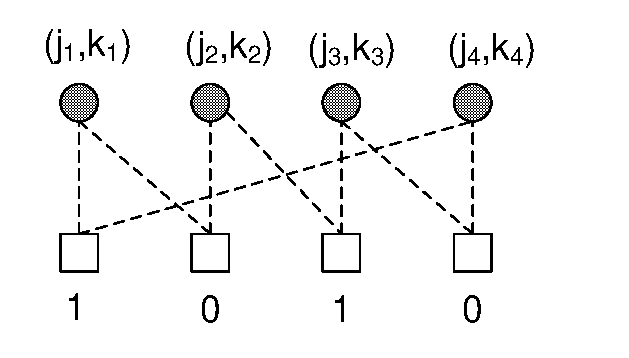
\includegraphics[width=2.75in,height=1.4in]{fig03.eps}
\caption{(Labelled) candidate (4,0) absorbing set}\label{Fig03}
\end{figure}
%By the vertex consistency condition, all the bit nodes that share
%a check node have different first indices. We may thus assume that
%$(j_1,k_1)$ and $(j_2,k_2)$ share a check in the row group $0$, as
%do $(j_3,k_3)$ and $(j_4,k_4)$, and that $(j_2,k_2)$ and
%$(j_3,k_3)$ share a check in the row group $1$, as do $(j_4,k_4)$
%and $(j_1,k_1)$, as shown in Figure \ref{Fig03}.
Note that the bits in this absorbing set along with their shared
checks constitute a cycle of length 8. Using
Lemma~\ref{cyclelemma} it follows that
\begin{equation}\label{eq1}
p\ell=j_3-j_2+j_1-j_4,
\end{equation}
for some integer $\ell$.

 \comment{Consider the matrix $M$,
\begin{equation}\label{matrixM}
M=(\sigma^{0j_1})^T(\sigma^{0j_2})(\sigma^{1j_2})^T(\sigma^{1j_3})(\sigma^{0j_3})^T(\sigma^{0j_4})(\sigma^{1j_4})^T(\sigma^{1j_1})~.
\end{equation}

By traversing the cycle in Figure~\ref{Fig03}, starting at the bit
node $(j_1,k_1)$ and then going into its neighboring check with
the label '0', we require that the matrix $M$ given in
\ref{matrixM} is an identity matrix. Since $M$ is itself a power
of $\sigma$, it is necessary that $M=\sigma^{p\ell}$, for some
$\ell$, where $\ell$ is an integer.

Moreover, since each component submatrix is a permutation matrix,
\begin{equation}\label{eq1a}
(\sigma^{\ell})^T=(\sigma^{\ell})^{-1} \end{equation} it further
follows that
\begin{equation}\label{eq1}
p\ell=j_3-j_2+j_1-j_4.
\end{equation}}

\comment{One solution to the last equation is $\ell = 0$, and
$j_1=1, j_3=p-1, j_2=2, j_4=p-2$. Since $(j_1,k_1)$ and
$(j_2,k_2)$ share a check in the row group $0$, it follows that
$k_1=k_2$, and likewise $k_3=k_4$. Since the column $k_2$ of
$\sigma^{j_2}$ and column $k_3$ of $\sigma^{j_3}$ have a non-zero
entry in the same row, it follows that
\begin{eqnarray*}
k_2+j_2 &\equiv & k_3+j_3 \mod p.
\end{eqnarray*}

Thus, the indices of the bit nodes participating in one such
absorbing set are $(j_1,k_1)$, $(j_2,k_1)$, $(j_3,[k_1-p+3]_p)$,
and $(j_4,[k_1-p+3]_p,)$, for $k_1$ chosen arbitrary in the
residue set$\mod p$, and where $[x]_p$ here and in the remainder
denotes a residue congruent to $x\mod p$.\hfill$\blacksquare$}

%It can be checked that for $\gamma=2$ the indicator function of
%every absorbing set is a codeword.
%\begin{lemma} The total number of $(4,0)$ absorbing sets in $C_{p,2}$ is XXXXX.
%\end{lemma}
%\noindent \textit{Proof:} It suffices to consider $l=-1,0,1$ in
%\ref{eq1}). First, for $l=0$ there are \hfill$\blacksquare$


\begin{lemma}\label{lemma40} There is a total of $p^2(p-1)^2$ $(4,0)$ (fully) absorbing sets in
the code described by $H_{p,2}$.
\end{lemma}
\noindent \textit{Proof:} Since $j_3-j_3+j_1-j_4 \in [-2(p-1),
2(p-1)]$ and $2(p-1)<2p$, it suffices to consider $\ell=1,0,-1$ in
(\ref{eq1}). Recall that $j_1,j_2,j_3,j_4$ in \eqref{eq1} all belong
to the set $\{0,\dots,p-1\}$.

First, for $\ell=1$, note that since $j_1+j_3$ is at most $2p-2$,
 $j_2+j_4$ is at most $p-2$. For each integer $s$ such that $0 \leq s \leq p-2$ there are
$(s+1)$ ways of assigning values to $j_2$ and $j_4$ to make
$j_2+j_4=s$. For each such $s$, there are $p-s-1$ ways of assigning
values to $j_1$ and $j_3$ to make $j_1+j_3=p+s$. Summing over all
choices of $s$ yields
\begin{equation}\label{sum401}\sum_{s=0}^{p-2}
(s+1)(p-s-1)=p(p-1)(p+1)/6\end{equation} as the total number of ways
of assigning values to $(j_1,j_2,j_3,j_4)$. By symmetry, for
$\ell=-1$ there are also $p(p-1)(p+1)/6$ ways of assigning values to
$(j_1,j_2,j_3,j_4)$.

For $\ell=0$, the sum $j_1+j_3$ is at most $2p-2$. For each $s$,
$0 \leq s \leq p-1$, there are $s+1$ ways of expressing $s$ as a
sum of an ordered pair $(j_1,j_3)$. For each $s$, $p-1 \leq s \leq
2p-2$, there are $2p-2-s+1$ ways of expressing it as a sum of an
ordered pair $(j_1,j_3)$, which is thus the same as the number of
assignments for $2p-2-s$.

It now suffices to consider $s$ where $0 \leq s \leq p-1$. Since
we are dealing with the $j_1+j_3 = j_2+j_4$ case, the numerical
assignment that makes $j_1=j_3 (j_4)$ or  $j_2=j_3 (j_4)$ needs to
be excluded by the edge consistency condition.  For $s$ odd and $0
\leq s \leq p-1$, each of these $s+1$ ordered pairs can be
assigned to $(j_1,j_3)$, and for each such assignment, $s-1$
ordered pairs can be assigned to $(j_2,j_4)$ (the two excluded
cases are the ones involving the assigned values to $j_1$ and
$j_3$). For $s$ even, for $s$ assignments out of possible $s+1$
(excluding the pair $(s/2,s/2)$) of $(j_1,j_3)$, $s-1$ ordered
pairs can be assigned to $(j_2,j_4)$. For the pair $(s/2,s/2)$
assigned to $(j_1,j_3)$, there are $s$ available assignments for
$(j_2,j_4)$. The total number of assignments for $l=0$ is
\begin{eqnarray}\label{sum402} 2\sum_{s=1,s \text{ odd}}^{p-2} (s+1)(s-1) + 2\sum_{s=2,s
\text{ even}}^{p-3} \left[s(s-1)+s\right] +
\left[(p-1)(p-2)+(p-1)\right] = 2p(p-1)(p-2)/3~.\end{eqnarray}

By summing~\eqref{sum402} with twice the expression
in~\eqref{sum401}, the total number of assignments for
$(j_1,j_2,j_3,j_4)$ is then $p(p-1)^2$. Since the column $k_1$ of
$\sigma^{1j_1}$ and the column $k_4$ of $\sigma^{1j_4}$ have a
non-zero entry in the same row, it follows by the parity check
consistency constraint
\begin{equation*}
k_1+j_1 \equiv k_4+j_4 \mod p~.
\end{equation*}
Likewise,
\begin{equation*}\begin{array}{cccc}
k_2+j_2 &\equiv &k_3+j_3,  \mod p\\
k_1 &\equiv &k_2 \mod p~, \text{ and}\\
 k_3 &\equiv &k_4\mod p~.
\end{array}\end{equation*}

Therefore, once the values of  $(j_1,j_2,j_3,j_4)$ are selected,
$k_1$ can be chosen in $p$ ways, and for each such assignment, the
values of $k_2$, $k_3$, and $k_4$, are then uniquely determined.
Hence, there are $p^2(p-1)^2$ different $(4,0)$ (fully) absorbing
sets.\hfill$\blacksquare$

\begin{corollary} The number of $(4,0)$ (fully) absorbing sets for
the code described by $H_{p,2}$ is $\Theta(n^{2})$, where $n$ is
the codeword length.
\end{corollary}
\noindent \textit{Proof:} Follows immediately from
Lemma~\ref{lemma40} and $n=p^2$.\hfill$\blacksquare$
% end of the comment

Note that $(4,0)$ absorbing sets are actually codewords, so  the
cycle code is dominated by low weight codewords. We now consider
$\gamma
> 2$, which leads to more interesting results. In particular, our results establish the
existence of minimal absorbing sets and minimal fully absorbing
sets, for which the number of bit nodes $a$ is \emph{strictly
smaller} than the minimum distance $d_{min}$ of the code.

\subsection{Absorbing sets of $H_{p,3}$}\label{theo12}

%\begin{lemma}\label{Lem1} The minimal absorbing set for $C_{p,3}$
%is a $(3,3)$ absorbing set.
%\end{lemma}
%\noindent \textit{Proof:}
We now turn to the proof of Theorem~\ref{theo1}(b), concerning the
sizes and numbers of minimal absorbing sets in $H_{p,3}$.

\comment{First observe that if there were to exist an unsatisfied
check node connected to three bit nodes participating in one such
absorbing set, there would necessarily exist a satisfied check
node connected to two of these three bit nodes. This however
violates the girth condition of the code. It is thus necessary
that all three bit nodes have a different unsatisfied check,
implying $b=3$. Moreover, these $a=3$ bits along with their shared
satisfied checks create a length 6 cycle.}

Let $G_{p,3}=(V,F,E)$ denote the Tanner graph of $H_{p,3}$. Let
$D$ be an $(a,b)$ absorbing set in $G_{p,3}$. Each bit node in $D$
has degree $3$ in $G_{p,3}$ and is required to have strictly more
neighbors in $\mathcal{E}(D)$ than in $\mathcal{O}(D)$.

\begin{figure}
\center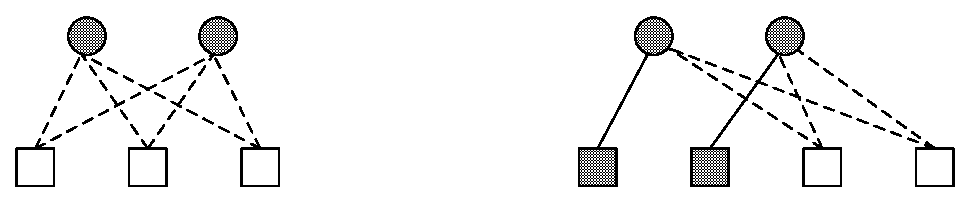
\includegraphics[width=3.45in,height=0.8in]{fig07.eps}
\caption{Candidate (2,b) absorbing sets}\label{Fig07}
\end{figure}
Suppose $a=2$. In $G_{p,3}$ an even number of edges from $D$
terminates in $\mathcal{E}(D)$. Thus either $b=0$ or $b=2$. These
correspond to the situations in Figure \ref{Fig07}. In either case
there would be a cycle of length 4 in $G_{p,3}$, which is false
\cite{fan}. Thus $a\geq 3$.

Suppose $a=3$. In $G_{p,3}$ an even number of edges from $D$
terminates in $\mathcal{E}(D)$. Thus either $b=1$ or $b=3$.
Suppose $b=1$. This must correspond to the form in Figure
\ref{Fig06},
\begin{figure}
\center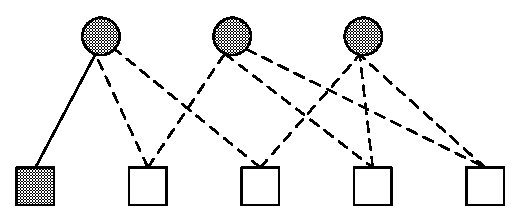
\includegraphics[width=1.9in,height=0.9in]{fig06a.eps}
\caption{Candidate (3,1) absorbing set}\label{Fig06}
\end{figure}
which again involves a cycle of length 4 in $G_{p,3}$, a
contradiction, \cite{fan}.

The remaining case with $a=3$ is $b=3$. In this case, each bit
node in $D$ would then connect to exactly one check node in
$\mathcal{O}(D)$ implying the unlabelled form of Figure
\ref{Fig05a}.
%\begin{figure}
%\vspace{0.1in}\hspace{0.4in}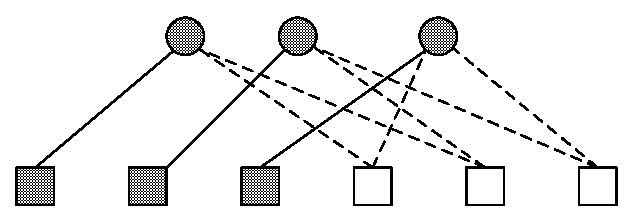
\includegraphics[width=2.5in,height=0.9in]{fig04.eps}
%\caption{Candidate (3,3) absorbing set}\label{Fig04}
%\end{figure}
Note that there is a cycle of length 6. Suppose that these $3$ bit
nodes are indexed as $(j_1,k_1)$, $(j_2,k_2)$ and $(j_3,k_3)$,
respectively, where $j_1,j_2$ and $j_3$ are distinct (by the edge
consistency) and $0 \leq j_1, j_2, j_3 \leq p-1$. Without loss of
generality assume that $(j_1,k_1)$ and $(j_2,k_2)$ share a check
in the row group $i_1$, $(j_2,k_2)$ and $(j_3,k_3)$ share a check
in the row group $i_2$, and that $(j_1,k_1)$ and $(j_3,k_3)$ share
a check in the row group $i_3$, where $i_1,i_2,i_3 \in \{0,1,2\}$
and are distinct by the vertex consistency condition. This
corresponds to the labelled representation in Figure \ref{Fig05a}.

In the remainder of the discussion we will first prove the
existence of a $(3,3)$ absorbing set. We will then show that these
$(3,3)$ absorbing sets are not fully absorbing sets. This result
will in turn imply the existence of $(4,2)$ fully absorbing sets,
which are thus minimal fully absorbing sets for $\gamma=3$.

\begin{figure}
\center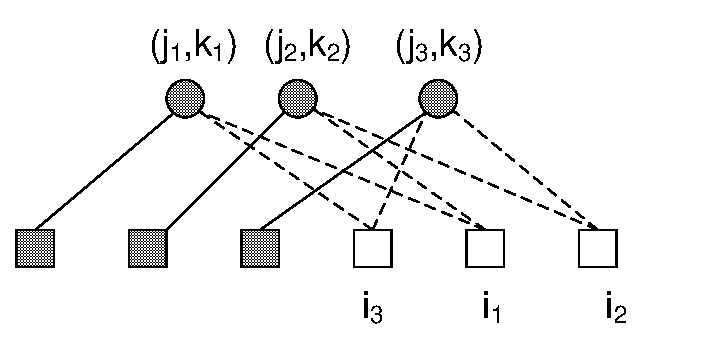
\includegraphics[width=2.7in,height=1.35in]{fig05a.ps}
\caption{(Labelled) candidate (3,3) absorbing set}\label{Fig05}
\end{figure}

Consider the length-6 cycle involving bit nodes $(j_1,k_1)$,
$(j_2,k_2)$, and $(j_3,k_3)$ as shown in Figure~\ref{Fig05}. Using
the cycle consistency condition  it follows that
\begin{equation}\label{eqpl}
p\ell=i_1(j_2-j_1)+i_2(j_3-j_2)+i_3(j_1-j_3).\end{equation}

\comment{By tracing the cycle in \ref{Fig05} we obtain that the
matrix $M_1$, where $M_1$ given by
\begin{equation}
M_1=(\sigma^{i_1j_1})^T(\sigma^{i_1j_2})(\sigma^{i_2j_2})^T(\sigma^{i_2j_3})(\sigma^{i_3j_3})^T(\sigma^{i_3j_1}),
\end{equation}
is an identity. Since $M_1$ has a non-zero entry on the main
diagonal, and is itself a power of $\sigma$, it is necessary that
$M_1=\sigma^{p\ell}$, for some $\ell$, where $\ell$ is an integer.

It thus follows that\begin{equation}\label{eqpl}
p\ell=i_1(j_2-j_1)+i_2(j_3-j_2)+i_3(j_1-j_3).\end{equation}}

By the symmetry of the absorbing set (see Figure \ref{Fig05}), we
may let $i_1=0$, $i_2=1$, and $i_3=2$. Since the column $k_1$ of
$\sigma^{2j_1}$ and column $k_3$ of $\sigma^{2j_3}$ have a
non-zero entry in the same row, it follows by the parity check
consistency (see~\eqref{cong}),
\begin{eqnarray}\label{eq12a}
k_1+2j_1 &\equiv & k_3+2j_3 \mod p.
\end{eqnarray}
Likewise,
\begin{eqnarray}\label{eq12b}
k_1 &\equiv& k_2   \mod p,\\
k_2 + j_2 &\equiv& k_3 +j_3  \mod p. \label{eq12c}
\end{eqnarray}
The existence of the solution for such a $(3,3)$ absorbing set is
given in the proof of Lemma~\ref{le11} below. \comment{For example,
a solution to this constraint is for $\ell=0, i_1=0, i_2=2, i_3=1$
and $j_1=1$, $j_2=(p-1)/2$, $j_3=p-2$. Since $(j_1,k_1)$ and
$(j_2,k_2)$ share a check in the row group $0$, it follows that
$k_1=k_2$. Since the column $k_1$ of $\sigma^{j_1}$ and column $k_3$
of $\sigma^{j_3}$ share a check in the row group 1, it follows that
\begin{eqnarray*}
k_1+j_1 &\equiv & k_3+j_3 \mod p.
\end{eqnarray*}

The indices of bit nodes participating in one such absorbing set
are $(k_1,j_1)$, $(k_1,j_2)$, and $([k_1-(p-3)]_p,j_3)$, for $k_1$
chosen arbitrary in the residue set$\mod p$.\hfill$\blacksquare$}

Even though the $(3,3)$ fully absorbing set seems plausible, care
must be taken with respect to a bit node \emph{outside} a
candidate fully absorbing set when this bit node also participates
in the unsatisfied checks. As we now show, such a $(3,3)$ fully
absorbing set cannot exist, though the existence of a $(3,3)$
absorbing set implies  a $(4,2)$ fully absorbing set.

\begin{figure}
\center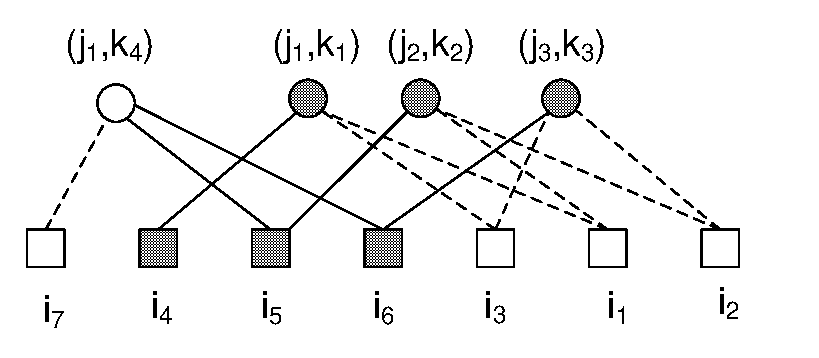
\includegraphics[width=2.7in,height=1.35in]{fig05c.eps}
\caption{Candidate (3,3) absorbing set (solid circles), with an
adjacent bit node (empty circle).}\label{Fig05a}
\end{figure}

Suppose first that a $(3,3)$ fully absorbing set exists. Since
$\gamma=3$, it is then necessary that no bit node outside of the
absorbing set participates in more than one unsatisfied check
adjacent to a $(3,3)$ absorbing set. Since $(j_1,k_1)$ and
$(j_3,k_3)$ share a check, $j_1 \neq j_3$. Consider the bit node
labelled $(j_1,k_4)$ that connects to $i_6$, as in Figure
\ref{Fig05a}. Since $i_3=2$ and $i_2=1$, $i_6$ has value 0 ($i_6
in\{0,1,2\}$ and distinct from $i_2,i_3$ by the vertex consistency
condition at $(j_3,k_3)$). Since $j_6=0$, it follows that $k_3=k_4$.
Note that likewise $i_5=2$ in Figure \ref{Fig05a}, since $i_1=0$,
and $i_2=1$, and using the vertex consistency condition at the bit
node $(j_3,k_3)$.

If the $(j_1,k_3)$ bit node does not also participate in the check
labelled with $i_5$ it would be necessary that $k_3+2j_1 \neq
k_2+2j_2 \mod p$, which is in contradiction with (\ref{eqpl})
through (\ref{eq12c}). Therefore the bit node $(j_1,k_3)$ shares
checks labelled with $i_5$ and $i_6$ with the bit nodes
$(j_2,k_2)$ and  $(j_3,k_3)$, respectively. This eliminates a
$(3,3)$ fully absorbing set for this configuration. This also now
implies a candidate $(4,2)$ fully absorbing set with bit nodes
$(j_1,k_1), (j_2,k_2)$, $(j_3,k_3)$ and $(j_1,k_3)$. Furthermore,
if a bit node labelled $(j_4,k_4)$ shares checks with the bit
nodes $(j_2,k_2)$ and $(j_,k_3)$ as above, $j_4=j_1$.

The cases where the bit node $(j_1,k_3)$ shares its remaining check,
which we label $i_7$, with one of $(j_1,k_1), (j_2,k_2)$, or
$(j_3,k_3)$ can be eliminated as we now show. By the vertex
consistency condition at the bit node $(j_1,k_3)$, $i_7=1$. By the
girth constraint, the bit node $(j_1,k_3)$ cannot share this check
with either $(j_2,k_2)$ or $(j_3,k_3)$. Since the bit node
$(j_1,k_1)$ already has the neighboring check whose label is
$i_4=1$, if the bit node $(j_1,k_3)$ also participates in this
check, it would imply the existence of a $(4,0)$ absorbing set,
which is impossible since the minimum distance of this code is 6,
\cite{helles}.

Therefore, in the resulting $(4,2)$ absorbing set, the unsatisfied
checks are labelled $i_4$ and $i_7$. Since $i_4=i_7=1$ no bit node
outside of this absorbing set can connect to both unsatisfied
checks, this $(4,2)$ configuration represents a fully absorbing
set.


It can be shown similarly that every $(4,2)$ fully absorbing set
has the shape as the unlabelled configuration in
Figure~\ref{Fig05a}, and that each can be obtained from an
underlying $(3,3)$ absorbing set. In particular, by the girth
condition, each unsatisfied check has degree 1 with respect to the
bits in the absorbing set (and these bits must be different by
definition of an absorbing set) and each neighboring satisfied
check has degree 2 with respect to the bits in the absorbing set.
To ensure that each bit node in the absorbing set has strictly
more satisfied than unsatisfied checks, it is further necessary
that the two bit nodes in the absorbing set with all neighboring
checks satisfied, each share a distinct check with one of the
remaining two bit nodes in the absorbing set, and one satisfied
check with each other. As a result, we arrive at the unlabelled
configuration in Figure~\ref{Fig05a}.


By symmetry, for each underlying $(3,3)$ absorbing set and for
each of the three choices of the labels of the resulting
unsatisfied check, there exists exactly one way of adjoining a
distinct fourth bit node that neighbors these unsatisfied checks.
Since the labels of the two unsatisfied checks are the same, each
resulting $(4,2)$ fully absorbing set comes from two different
$(3,3)$ underlying configurations.

 We complete the section with the following result.
\begin{lemma}\label{le11} The total number of $(3,3)$ absorbing sets and $(4,2)$ fully absorbing sets
in the Tanner graph described by $H_{p,3}$ is $p^2(p-1)$, and
$3p^2(p-1)/2$, respectively.
\end{lemma}
\noindent \textit{Proof:} It suffices to consider $\ell=-1,0,1$ in
(\ref{eqpl}) with $i_1=0$, $i_2=1$ and $i_3=2$.

For $\ell=0$, $2j_1=j_2+j_3$. For each value of $j_1$, $1 \leq j_1
\leq (p-1)/2$, there are $2j_1$ ways of assigning values to
$(j_1,j_2,j_3)$ (the cases where two of $j_1$,$j_2$ and $j_3$ are
the same have to be excluded by the edge consistency condition).
Likewise, for each $j_1$ where $(p+1)/2 \leq j_1 \leq p-2$ there
are $2(p-1-j_1)$ ways of assigning values to $(j_1,j_2,j_3)$. For
each assignment there are $p$ ways to assign values to
$(k_1,k_2,k_3)$ to ensure the validity of
(\ref{eq12a})-(\ref{eq12c}). In all, there is a total of
\[p\left[\sum_{j_1=1}^{(p-1)/2} 2j_1 + \sum_{j_1=(p+1)/2}^{p-2}
2(p-1-j_1)\right] = \frac{p(p-1)^2}{2}\] such assignments, each
describing a different $(3,3)$ absorbing set.

Likewise, for $\ell=1$ (and for $\ell=-1$ by symmetry) we require
$p+(j_2+j_3)=2j_1$. Thus $s=(j_2+j_3)$ is at most $p-2$ and odd.
For each such $s$, there are $s+1$ ways to assign the values to
$j_1,j_2$ and $j_3$, and for each such assignment, there are $p$
ways to assign values to $(k_1,k_2,k_3)$ to ensure the validity of
(\ref{eq12a})-(\ref{eq12c}). The total number of ways to select a
(3,3) absorbing set in this case is
\[
p\left[\sum_{s=1, s \text{
odd}}^{p-2}(s+1)\right]=\frac{p(p-1)(p+1)}{4}~.
\]

The total number of $(3,3)$ absorbing sets is thus $p^2(p-1)$.

Depending on which two of these three bit nodes the remaining bit
node $(j_4,k_4)$ (in the $(4,2)$ fully absorbing set) shares a
(satisfied) check with, we may assign $(j_4,k_4)$ in three
different ways. Note that in this way we have counted each $(4,2)$
set twice. Hence there are $3p^2(p-1)/2$ distinct $(4,2)$ fully
absorbing sets. \hfill$\blacksquare$

%\begin{corollary} The number of $(3,3)$ absorbing sets in
%$C_{p,3}$ is $O(n^{3/2})$, where $n$ is the codeword length.
%\end{corollary} \noindent \textit{Proof:}

Since the codeword length $n$ is $p^2$, the result of Lemma
\ref{le11} implies Theorem~\ref{theo2} for $\gamma=3$, that is, the
number of minimal absorbing sets as well as the number of minimal
fully absorbing sets grows as $\Theta(n^{3/2})$. Observe that we
have proved  the existence of the minimal fully absorbing sets of
size $(4,2)$. By comparison, the minimum distance of the
$C_{p,\gamma}$ code is $6$, \cite{helles}.

\subsection{Absorbing sets of $H_{p,4}$}\label{theo14}
%\subsubsection{Subsubsection Heading Here}
%Subsubsection text here.



In order to establish that $(6,4)$ (fully) absorbing sets are
minimal for $H_{p,4}$, we will first show that $(a,b)$ absorbing
sets for $a < 6$ do not exist.

\comment{First, the condition $a<4$ is not possible as it would
violate the girth condition. For $a=4$, if $b<4$, there would
exist a bit node sharing at least two satisfied checks with some
other bit node in the absorbing set. If $b>4$, there would exist a
bit node in the absorbing set having more unsatisfied that
satisfied checks, which is not possible by definition. Thus, for
$a=4$, the only nontrivial candidate absorbing set is a $(4,4)$
absorbing set. }


Let $D$ denote an $(a,b)$ absorbing set in $G_{p,4}=(V,F,E)$, the
Tanner graph of $H_{p,4}$. If $a=2$ (respectively $3$) then at
least $6$ (respectively $9$) edges from $D$ in $G_{p,4}$ terminate
in $\mathcal{E}(D)$, which implies the existence of a cycle of
length 4 in $G_{p,4}$, which is false \cite{fan}. Thus, $a \geq
4$.

Suppose $a=4$. The number of edges from $D$ in $G_{p,4}$ that
terminate in $\mathcal{E}(D)$ must be 12, 14, or 16, corresponding
to the cases $b$ = 4, 2, or 0, respectively. No check node in
$\mathcal{E}(D)$ can connect to all four of the bit nodes in $D$,
else there would need to be a cycle of length 4 in $G_{p,4}$,
which is false \cite{fan}. Thus, each check node in
$\mathcal{E}(D)$ connects to exactly two of the bit nodes in $D$.
There are $6$ pairs of nodes in $D$. Thus we must have $b=4$. The
following lemma establishes that such sets do not exist for large
enough prime $p$.


\begin{lemma}\label{Lem2} For $p>7$, the Tanner graph family $G_{p,4}$
does not contain any $(4,4)$ absorbing sets.
\end{lemma}
\noindent \textit{Proof:} No check node satisfied with respect to
the absorbing set has degree $> 2$, as otherwise there would exist
two bit nodes that share two distinct check nodes, which is not
possible by the girth condition \cite{fan}. Similarly, all bit
nodes in an absorbing set have distinct unsatisfied check nodes.

%\begin{figure}\hspace{1.0in}
%\begin{picture}(100,150)(0,0)
%\put(10,50){\line(1,0){60}} \put(10,110){\line(1,0){60}}
%\put(10,50){\line(0,1){60}} \put(70,50){\line(0,1){60}}
%\put(10,50){\line(1,1){60}} \put(10,110){\line(1,-1){60}}
%\put(0,40){{$(j_4,k_4)$}} \put(60,120){{$(j_2,k_2)$}}
%\put(0,120){{$(j_1,k_1)$}} \put(60,40){{$(j_3,k_3)$}}
%%\put(255,205){{$c_1^0(11)$='1'}}
%\put(0,80){{$i_4$}} \put(75,80){{$i_2$}} \put(40,120){{$i_1$}}
%\put(40,40){{$i_3$}} \put(31,90){{$i_5$}} \put(31,65){{$i_6$}}
%\end{picture}
%\caption{Depiction of the (4,4) set}
%\end{figure}
\begin{figure}
\center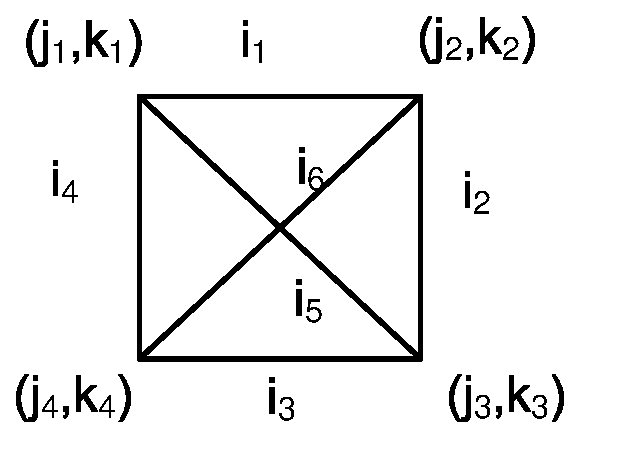
\includegraphics[width=2.65in,height=1.5in]{Drawing10_1.eps}
\caption{Depiction of the candidate (4,4) set} \label{fig44}
\end{figure}

Since each bit node in the absorbing set shares exactly 3
satisfied check nodes with other bit nodes in the absorbing set,
we can view the absorbing set as shown in Figure \ref{fig44} where
each (labelled) vertex represents a distinct bit node and each
(labelled) edge represents a check node in which the bit nodes
associated with its endpoints participate.

\comment{By the edge consistency condition all $j_1$ through $j_4$
are different. Since the column $k_1$ of $\sigma^{i_1j_1}$ and
column $k_2$ of $\sigma^{i_1j_2}$ have a non-zero entry in the
same row, it follows that
\begin{eqnarray*}
k_1+i_1j_1 &\equiv & k_2+i_1j_2 \mod p
\end{eqnarray*}

Likewise, for $i_2$ through $i_6$ we obtain
\begin{eqnarray*}
k_2+i_2j_2 &\equiv& k_3+i_2j_3 \mod p, \\
k_3+i_3j_3 &\equiv& k_4+i_3j_4 \mod p, \\
k_1+i_4j_1 &\equiv& k_4+i_4j_4 \mod p, \\
k_1+i_5j_1 &\equiv& k_3+i_5j_3 \mod p, \text{and}\\
k_2+i_6j_2 &\equiv& k_4+i_6j_4 \mod p.
\end{eqnarray*}}

Without loss of generality we may let $i_1=x$, $i_2=y$ and
$i_4=z$, where $x,y,z \in \{0,1,2,3\}$ and distinct by the vertex
consistency condition at $(j_1,k_1)$. Then, by propagating the
vertex consistency conditions at each remaining vertex, and
exploiting the symmetry, it suffices to consider
$(i_1,i_2,i_3,i_4,i_5,i_6)$ either $(x,y,x,y,z,z)$ or
$(x,y,x,y,z,w)$ where $x,y,z,w \in \{0,1,2,3 \}$ and are distinct.

For the case $(i_1,i_2,i_3,i_4,i_5,i_6)$ = $(x,y,x,y,z,z)$, we
establish the following conditions based on the cycles within the
graph in Figure \ref{fig44}:
\begin{equation}\label{eq44a}\begin{array}{ccccc}
p\ell_1&=&x(j_2-j_1)+y(j_3-j_2)+z(j_1-j_3),& \\
p\ell_2&=&x(j_2-j_1)+z(j_4-j_2)+y(j_1-j_4),&\text{and}\\
p\ell_3&=&x(j_4-j_3)+y(j_1-j_4)+z(j_3-j_1).&
\end{array}\end{equation}
for some integers $\ell_1,\ell_2$ and $\ell_3$.

By adding and subtracting the conditions in~\eqref{eq44a}, it
follows that
\begin{equation}\label{eq44b}\begin{array}{ccccc}
p\ell_1'&=&(y-z)(j_3+j_4-j_1-j_2),&\\
p\ell_2'&=&(x-z)(j_2+j_3-j_1-j_4),&\text{and}\\
p\ell_3'&=&(x-y)(j_2+j_4-j_1-j_3).&
\end{array}\end{equation}

\noindent for some integers $\ell_1',\ell_2'$ and $\ell_3'$. Since
$x,y,z$ are distinct, ~\eqref{eq44b} implies that $j$'s would have
to be the same, which contradicts the edge consistency constraint.

For the case $(i_1,i_2,i_3,i_4,i_5,i_6)$ = $(x,y,x,y,z,w)$, again
based on the cycle structure in Figure \ref{fig44}, we have that
\begin{equation}\label{eq44c}\begin{array}{ccccc}
p\ell_1&=&x(j_2-j_1)+y(j_3-j_2)+z(j_1-j_3)&,&{}\\
p\ell_2&=&x(j_2-j_1)+w(j_4-j_2)+y(j_1-j_4)&,&\text{and}\\
p\ell_3&=&x(j_4-j_3)+y(j_1-j_4)+z(j_3-j_1)&.&{}
\end{array}\end{equation}
for some integers $\ell_1,\ell_2$ and $\ell_3$.

We let $u_1 \asn j_2-j_1$, $u_2 \asn j_3-j_1$, and $u_3 \asn
j_4-j_1$. By the edge consistency condition, all of $u_1$, $u_2$,
and $u_3$ are non-zero. Substituting $u_1$, $u_2$ and $u_3$ in
~\eqref{eq44c} and then expressing $u_2$ and $u_3$ in terms of
$u_1$, one arrives at the condition
\begin{equation}\label{eq23}
(z-x)(w-y)+(z-y)(w-x) \equiv 0 \mod p.
\end{equation}

It can be easily verified that this condition can not hold for any
choice of $x,y,z,w$, where $x,y,z,w \in \{0,1,2,3 \}$ and are
distinct for $p>7$. There are $4!=24$ ways of assigning numerical
values to $(x,y,z,w)$. The expression in~\eqref{eq23} is at most $7$
in absolute value for such $x,y,z$, and $w$.  Substituting each
numerical assignment $(x,y,z,w)$ yields possible choices of prime
$p$ for which the expression in~\eqref{eq23} becomes zero $\mod p$.
The condition~\eqref{eq23} holds for $p \in \{2,5,7\}$. Therefore,
for $p>7$, $G_{p,\gamma}$ does not contain $(4,4)$ absorbing
sets.\hfill$\blacksquare$

%(the solutions exist for $p \in \{2,5,7\}$

 We next show that $(5,b)$
absorbing sets do not exist for the parameter $p$ large enough. In
particular we will establish a congruential constraint involving the
labels of the edges emanating from the bits in the absorbing set
that cannot hold for $p$ large enough.
\begin{lemma}\label{Lem3} For $p>19$, the Tanner graph family $G_{p,4}$
does not contain any $(5,b)$ absorbing sets.
 \end{lemma}

\noindent \textit{Proof:} Since each bit node in the absorbing set
has at most one neighboring unsatisfied check node, it follows that
$b \leq 5$. Observe that the number of bit nodes with 3 satisfied
and 1 unsatisfied check nodes is even, and thus $b$ is even. First
$b>0$ by the minimum distance, $d_{min}\geq 8$ of the code,
\cite{helles}. If $b=2$ and all satisfied check nodes had degree 2,
such an absorbing set would contain a $(4,4)$ absorbing set, which
by Lemma \ref{Lem2} does not exist. A degree-4 satisfied check node
would violate the girth condition.


We are thus left with analyzing $b=4$ with all satisfied check
nodes of degree 2. Note that by the girth condition, all
unsatisfied checks have degree 1 with respect to the bits in the
absorbing set. Therefore, this candidate absorbing sets contains 1
bit node with all checks satisfied and 3 bit nodes each with 3
satisfied and 1 unsatisfied check. The only way that such an
absorbing set could exist (and not have double edges) is if one
has the configuration shown in Figure \ref{fig52}, where the
vertices represent bit nodes and edges represent their satisfied
check nodes.
%we have that $i_1$ connect $(k_1,j_1)$ and
%$(k_2,j_2)$, $i_2$ connect $(k_1,j_1)$ and $(k_3,j_3)$, $i_3$
%connect $(k_1,j_1)$ and $(k_4,j_4)$, $i_4$ connect $(k_1,j_1)$ and
%$(k_5,j_5)$, $i_5$ connect $(k_2,j_2)$ and $(k_3,j_3)$, $i_6$
%connect $(k_2,j_2)$ and $(k_4,j_4)$, $i_7$ connect $(k_3,j_3)$ and
%$(k_5,j_5)$, and $i_8$ connect $(k_4,j_4)$ and $(k_5,j_5)$, as

%\begin{figure}\hspace{1.0in}
%\begin{picture}(100,150)(0,0)
%\put(10,50){\line(1,0){60}} \put(10,110){\line(1,0){60}}
%\put(10,50){\line(0,1){60}} \put(70,50){\line(0,1){60}}
%\put(10,50){\line(1,1){60}} \put(10,110){\line(1,-1){60}}
%\put(0,40){{$(j_4,k_4)$}} \put(60,120){{$(j_2,k_2)$}}
%\put(0,120){{$(j_1,k_1)$}} \put(60,40){{$(j_3,k_3)$}}
%%\put(255,205){{$c_1^0(11)$='1'}}
%\put(0,80){{$i_4$}} \put(75,80){{$i_2$}} \put(40,120){{$i_1$}}
%\put(40,40){{$i_3$}} \put(31,90){{$i_5$}} \put(31,65){{$i_6$}}
%\end{picture}
%\caption{Depiction of the candidate (5,2) set}
%\end{figure}

\begin{figure}
\center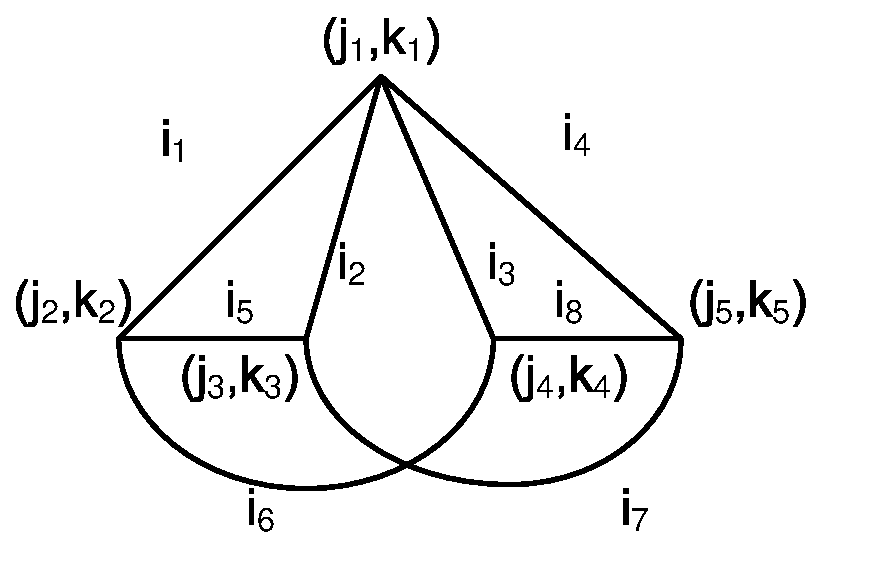
\includegraphics[width=3.0in,height=1.8in]{Drawing22_1.eps}
\caption{Depiction of the candidate (5,4) set} \label{fig52}
\end{figure}

Since $i_1$, $i_2$, $i_3$ and $i_4$ are all distinct elements of
the set $\{0,1,2,3\}$, by the vertex consistency condition, and by
the symmetry of the candidate configuration in Figure~\ref{fig52},
we may assume that $i_1=0$. We let $x \asn i_2$, $y \asn i_3$ and
$z \asn i_4$, where $x,y,z \in \{1,2,3 \}$ and distinct. By
propagating possible values of the labels for remaining edges,
while maintaining vertex consistency conditions, it follows that
$(i_1,i_2,i_3,i_4,i_5,i_6,i_7,i_8)$ is either $(0,x,y,z,y,z,0,x)$
or $(0,x,y,z,z,x,y,0)$.

For $(i_1,i_2,i_3,i_4,i_5,i_6,i_7,i_8)$ = $(0,x,y,z,y,z,0,x)$, and
for each edge and its endpoints in Figure~\ref{fig52}, we write the
parity check consistency constraint, in terms of $x$, $y$ and $z$,
\begin{subequations}\label{eq52a}\begin{eqnarray}
\label{eq52a1}k_1 &\equiv& k_2 \mod p,\\
\label{eq52a2}k_3 &\equiv& k_5 \mod p,\\
\label{eq52a3}k_1+xj_1 &\equiv& k_3+xj_3 \mod p, \\
\label{eq52a4}k_1+yj_1 &\equiv& k_4+yj_4 \mod p, \\
\label{eq52a5}k_1+zj_1 &\equiv& k_5+zj_5 \mod p, \\
\label{eq52a6}k_2+yj_2 &\equiv& k_3+yj_3 \mod p, \\
\label{eq52a7}k_2+zj_2 &\equiv& k_4+zj_4 \mod p, \text{and}\\
\label{eq52a8}k_4+xj_4 &\equiv& k_5+xj_5 \mod p.
\end{eqnarray}\end{subequations}

This last system simplifies to
\begin{equation}\label{eq52b}\begin{array}{llllll}
k_1+xj_1 &\equiv& k_3+xj_3 \mod p,& {}&\text{(from \eqref{eq52a3})}\\
k_1+yj_1 &\equiv& k_4+yj_4 \mod p,& {}&\text{(from \eqref{eq52a4})}\\
k_1+zj_1 &\equiv& k_3+zj_5 \mod p,& {}&\text{(from \eqref{eq52a2} and \eqref{eq52a5})}\\
k_1+yj_2 &\equiv& k_3+yj_3 \mod p,& {}&\text{(from \eqref{eq52a1} and \eqref{eq52a6})}\\
k_1+zj_2 &\equiv& k_4+zj_4 \mod p, &\text{and}&\text{(from \eqref{eq52a1} and \eqref{eq52a7})}\\
k_4+xj_4 &\equiv& k_3+xj_5 \mod p.&{}&\text{(from \eqref{eq52a2} and
\eqref{eq52a8})}
\end{array}\end{equation}

Thus
\begin{subequations}\begin{eqnarray}
\label{eq52s1}k_1-k_3 &\equiv x(j_3-j_1) \equiv z(j_5-j_1) \equiv
y(j_3-j_2) &
\mod p\\
\label{eq52s2}k_1-k_4 &\equiv y(j_4-j_1) \equiv z(j_4-j_2) &
\mod p\\
\label{eq52s3}k_3-k_4 &\equiv x(j_4-j_5) &\mod p.
\end{eqnarray}\end{subequations}

 We let $u_1 \asn j_3 -j_1$, $u_2\asn j_4 -j_1$, $u_3 \asn j_4
-j_1$, and $u_4 \asn j_3 -j_2$. Note that by the edge consistency
condition, all of $u_1$, $u_2$, $u_3$, and $u_4$ are non-zero.

We then obtain
\begin{equation}\begin{array}{cccccc}
xu_1 &\equiv& zu_3 & \mod p & \text{(from \eqref{eq52s1}),} \\xu_1
&\equiv& yu_4 & \mod p & \text{(from \eqref{eq52s1}),}\\
yu_2 &\equiv& z(u_2-u_1+u_4)& \mod p & \text{(from \eqref{eq52s2}),}
\\x(u_2-u_3)
&\equiv& yu_2-xu_1 & \mod p & \text{from
$k_3-k_4=(k_1-k_4)-(k_1-k_3)$ and }\\{}&{}&{}&{}& \text{substituting
from \eqref{eq52s3},\eqref{eq52s2},\eqref{eq52s1}),resp.}
\end{array}\end{equation}

This last system can be rewritten as
\begin{equation}\label{sys52a}
\left[ \begin{array}{ccccccc} x & 0 & 0 & -y\\
x & 0 & -z &0\\
-z & z-y &0 & z\\
-x & y-x & x & 0
\end{array}\right] \left[\begin{array}{c}
u_1\\u_2\\u_3\\u_4 \end{array}\right] \equiv
\left[\begin{array}{c}0\\0\\0\\0\end{array}\right] \mod p~.
\end{equation}

Therefore, the determinant of the matrix multiplying the
(non-zero) vector $\left[u_1 u_2 u_3 u_4\right]^{t}$ in
~\eqref{sys52a} is itself zero, which simplifies to
\begin{equation}\label{eq5a}
xy(z-x)(z-y)-z^2(x-y)^2 \equiv 0 \mod p,
\end{equation}

Since $x,y,z \in \{1,2,3\}$ and distinct we consider all $3!=6$
assignment for $(x,y,z)$, and for each we evaluate the left had side
expression in~\eqref{eq5a}. Note that for distinct $x,y,z \in
\{1,2,3\}$ , this expression is at most $19$ in absolute value, and
therefore the constraint in ~\eqref{eq5a} does not have a solution
for $p>19$ for distinct $x,y,z \in \{1,2,3\}$. (Solutions exist for
$p=5,11$ and $19$, which can be verified by direct numerical
substitution).

For $(i_1,i_2,i_3,i_4,i_5,i_6,i_7,i_8)$ = $(0,x,y,z,z,z,y,0)$ we
likewise establish the constraints as in \eqref{eq52a} and
\eqref{eq52b}. We again let $u_1 \asn j_3 -j_1$, $u_2\asn j_4
-j_1$, $u_3 \asn j_4 -j_1$, and $u_4 \asn j_3 -j_2$, and obtain
\begin{equation}\label{sys52b}
\left[ \begin{array}{ccccccc} 0 & y & -z & 0\\
x & y-x & 0 & -x\\
x & 0 &0 & -z\\
y-x & y & -y & 0
\end{array}\right] \left[\begin{array}{c}
u_1\\u_2\\u_3\\u_4 \end{array}\right] \equiv
\left[\begin{array}{c}0\\0\\0\\0\end{array}\right] \mod p~.
\end{equation}

Since the entries in  $\left[u_1 u_2 u_3 u_4\right]^{t}$ are all
non-zero, it follows that the determinant of the matrix
in~\eqref{sys52b} is zero. Simplifying the expression for the
determinant yields again the condition in \eqref{eq5a}. Therefore
for $p>19$, (5,4) absorbing sets do not exist.\hfill$\blacksquare$

\comment{ and likewise for $i_8=0$ we let $x=i_2=i_6$, $y=i_3=i_7$
and $z=i_4=i_5$. Note that now $k_1=k_2$ and $k_4=k_5$ and
\begin{eqnarray*}
k_1+xj_1 &\equiv& k_3+xj_3 \mod p, \\
k_1+yj_1 &\equiv& k_4+yj_4 \mod p, \\
k_1+zj_1 &\equiv& k_5+zj_5 \mod p, \\
k_2+zj_2 &\equiv& k_3+zj_3 \mod p, \\
k_2+xj_2 &\equiv& k_4+xj_4 \mod p, \text{and}\\
k_3+yj_3 &\equiv& k_5+yj_5 \mod p.
\end{eqnarray*}

where $x,y,z\in \{1,2,3\}$ and distinct.}

\comment{In both cases, after some algebra we arrive at
\begin{equation}\label{eq5a}
xy(z-x)(z-y)-z^2(x-y)^2 \equiv 0 \mod p,
\end{equation}
which does not have a solution for $p>19$ for distinct $x,y,z \in
\{1,2,3\}$.\hfill$\blacksquare$ %\footnote{As a side remark, we note that equation
%(\ref{eq5a}) does have a solution for $p \in \{5,11,19$\}.}
}
%No 4 deg. checks. dmin is 8.
%\begin{remark}

We can now proceed with the analysis of $(6,b)$ absorbing sets.
Since the number of bit nodes with 3 satisfied and 1 unsatisfied
check node is even, $b$ is even. First, $b=0$ is not possible
since $d_{min} \geq 8$ \cite{helles}. The following lemma
considers $b=2$.

\comment{ Observe that there cannot be a check of degree 4 with
respect to the bits in a $(6,b)$ absorbing set, as otherwise the
girth condition would be violated. As a result, in the remainder
of the analysis we will assume that all checks that have even
number of bit node neighbors in a $(6,b)$ absorbing set have
degree 2 with respect to the absorbing set. Moreover, since
$d_{min} \geq 8$ \cite{helles} and since all bit nodes in the
$(6,b)$ absorbing set have at most one unsatisfied check (with
respect to the absorbing set), it suffices to consider $b$ even
and positive.}
%\end{remark}

\begin{lemma}\label{Lem4} For $p>19$, the Tanner graph family $G_{p,4}$ does not contain any $(6,2)$ absorbing sets.
\end{lemma}

\noindent \textit{Proof:}
%\begin{figure}\hspace{1.0in}
%\begin{picture}(100,150)(0,0)
%\put(10,50){\line(1,0){60}} \put(10,110){\line(1,0){60}}
%\put(10,50){\line(0,1){60}} \put(70,50){\line(0,1){60}}
%\put(10,50){\line(1,1){60}} \put(10,110){\line(1,-1){60}}
%\put(0,40){{$(j_4,k_4)$}} \put(60,120){{$(j_2,k_2)$}}
%\put(0,120){{$(j_1,k_1)$}} \put(60,40){{$(j_3,k_3)$}}
%%\put(255,205){{$c_1^0(11)$='1'}}
%\put(0,80){{$i_4$}} \put(75,80){{$i_2$}} \put(40,120){{$i_1$}}
%\put(40,40){{$i_3$}} \put(31,90){{$i_5$}} \put(31,65){{$i_6$}}
%\end{picture}
%\begin{picture}(100,150)(0,0)
%\put(10,50){\line(1,0){60}} \put(10,110){\line(1,0){60}}
%\put(10,50){\line(0,1){60}} \put(70,50){\line(0,1){60}}
%\put(10,50){\line(1,1){60}} \put(10,110){\line(1,-1){60}}
%\put(0,40){{$(j_4,k_4)$}} \put(60,120){{$(j_2,k_2)$}}
%\put(0,120){{$(j_1,k_1)$}} \put(60,40){{$(j_3,k_3)$}}
%%\put(255,205){{$c_1^0(11)$='1'}}
%\put(0,80){{$i_4$}} \put(75,80){{$i_2$}} \put(40,120){{$i_1$}}
%\put(40,40){{$i_3$}} \put(31,90){{$i_5$}} \put(31,65){{$i_6$}}
%\end{picture}
%\caption{Depiction of the candidate (6,2) sets}
%\end{figure}
\begin{figure}
\center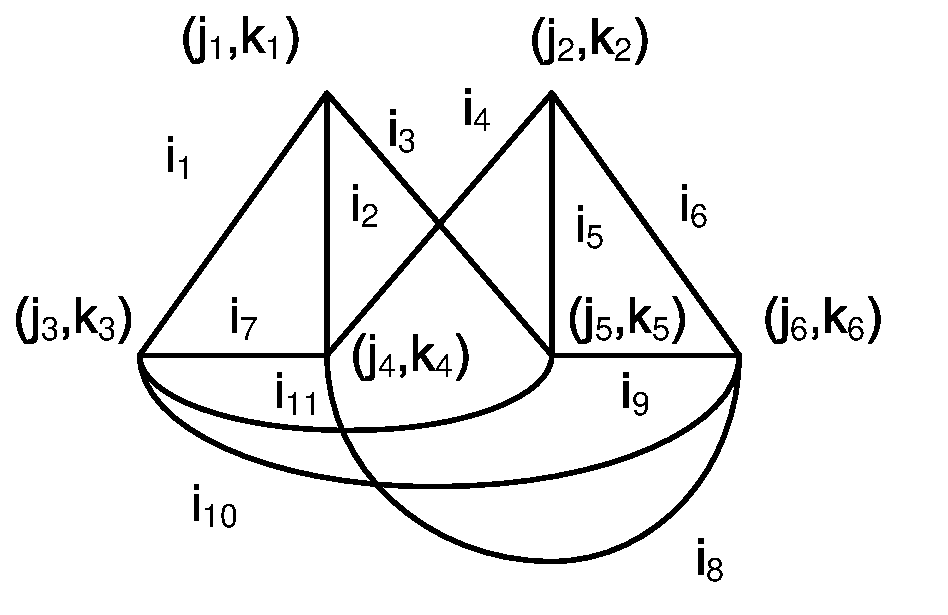
\includegraphics[width=2.8in,height=1.8in]{Drawing30_2.eps}
\center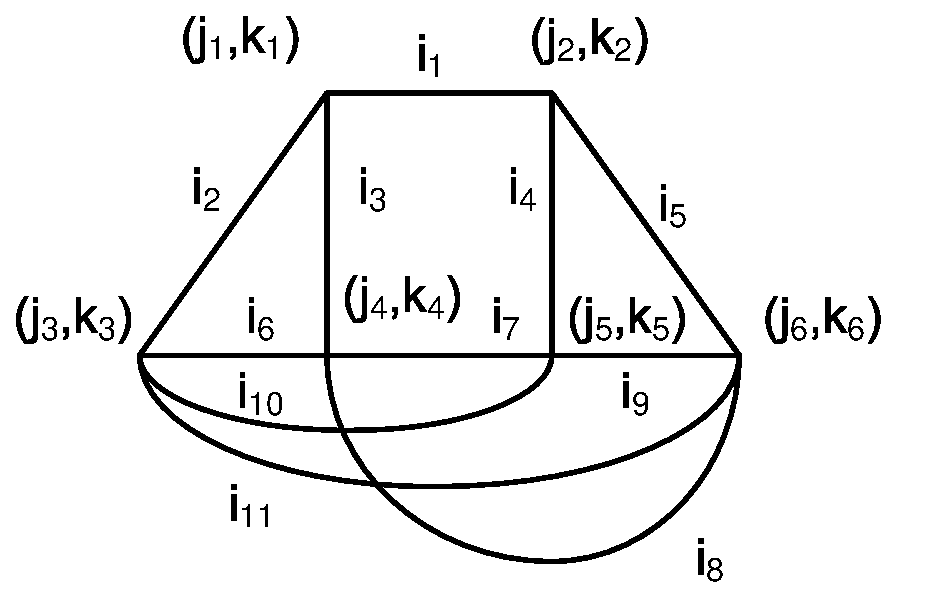
\includegraphics[width=2.8in,height=1.8in]{Drawing32_1.eps}\hspace{0.3in}
\caption{Depiction of the candidate (6,2) sets.} \label{fig62}
\end{figure}

%%%%%%%%%%%%%%%%%%%%%%%%%%%%%%
%%%%%%  NEW STUFF 20/8
%%%%%%%%%%%%%%%%%%%%%%%%%%%%%%
\comment{We first claim that there is no check node of degree at
least 4 with respect to the bit nodes in the absorbing set.
Indeed, if this were to occur, there would exist at least 2 bit
nodes in the absorbing set with all check nodes satisfied and with
a shared check node of degree at least 4. They would necessarily
share another check node, which is not possible by the girth
condition \cite{fan}.

We can now focus on the case where all satisfied check nodes with
respect to the absorbing set have degree 2. By requiring that each
vertex corresponding to a bit node in the absorbing set has either
3 or 4 outgoing edges, and that there are no parallel edges, it
follows that there are 2 possible configurations, as shown in
Figure \ref{fig62}, that relate bit nodes in the absorbing set
(vertices) and their shared satisfied checks (edges). Note that it
is apriori possible to have an unsatisfied check of degree 3 with
respect to the bit nodes in the absorbing set. This condition is
not a part of Figure\ref{fig62}.}

We first claim that there is no check node of degree at least 3
with respect to the bit nodes in the absorbing set. Let us first
suppose that there exists one such check node and that it has an
even degree with respect to the bit nodes in the absorbing set.
Since we are considering an absorbing set with 6 bit nodes, such a
check node would have degree either 4 or 6 with respect to the bit
nodes in the absorbing set. Each bit node in the absorbing set has
at least 3 (out of 4) neighboring satisfied checks. If this
satisfied check is of degree 6, there would exist 2 bit nodes in
the absorbing set which would share an additional satisfied check.
This situation would imply the existence of a cycle of length 4,
which is impossible by the girth condition.

Suppose now that this satisfied check has degree 4. Each bit node
that participates in this check has at least 2 more neighboring
satisfied checks, which it then necessarily must share with the
remaining two bit nodes in the absorbing set that themselves do
not participate in this degree-4 check. If there exists a bit node
that participates in this degree-4 check and has all checks
satisfied, it then shares its remaining neighboring check with one
of the bit nodes with which it already shares a check. This
situation violates the girth constraint. If all bit nodes in the
absorbing set that participate in this degree-4 check have 3
satisfied and 1 unsatisfied check, three of them would have to
participate in the same unsatisfied check to make the total number
of unsatisfied checks be 2. This again violates the girth
condition.

Therefore, all satisfied checks with respect to the bit nodes in
the absorbing set have degree 2. Suppose there exists a check node
that is unsatisfied with respect to the bits in the absorbing set
and that has degree bigger than 1. If such a check node has degree
5, there would necessarily exist 2 bit nodes in the absorbing set
that share this degree-5 check and another satisfied check, which
is impossible by the girth condition.

Suppose that there exists 2 degree-3 checks incident to the bit
nodes in the absorbing set. First, these degree-3 checks do not
have any neighboring bit nodes in common since we require that
each bit node has at most 1 unsatisfied check. We can then group
the bit nodes in the absorbing set into two disjoint groups, each
of size 3, such that the bits in the same group share the same
degree-3 check. Consider a bit node in, say, the first group. It
shares its remaining 3 (satisfied) checks with one of each bit
nodes in the second group. The same is true with the other two bit
nodes in the first group, namely they too share their remaining 3
(satisfied) checks with the bit nodes in the second group.
Therefore, there exist two bit nodes in the first group and two
bit nodes in the second group such that any two share a distinct
check. This configuration is not possible by Lemma 5 for $p>7$.

Suppose now there exists one unsatisfied check of degree 3 with
respect to the bit nodes in the absorbing set. The remaining
unsatisfied check then has degree 1 with respect to the bit nodes
in the absorbing set, and the neighboring bit nodes in the
absorbing set of these two unsatisfied checks are different. There
are two bit nodes in the absorbing set that have all checks
satisfied. Partition the bit nodes in the absorbing set into three
groups: the first group contains the three  bit nodes that share a
degree-3 unsatisfied check, the second group contains the one bit
node that has one unsatisfied check, and the third group contains
the two bit nodes that have all four checks satisfied. Each of the
three bit nodes in the first group has one unsatisfied and three
satisfied checks and thus it shares a satisfied check with each of
the bit nodes in the second and third group since it cannot share
a satisfied check with another bit node in the first group by the
girth condition. The bit node in the second group also has one
unsatisfied and three satisfied checks, and the latter are shared
then with bit nodes in the first group. The two bit nodes in the
third group have all four checks satisfied, the three of which
they each share with each of the bit nodes in the first group.
Since all three satisfied checks of the bit node in the second
group are used up with the checks it shares with the bit nodes in
the first group, the two bit nodes in the third group share a
satisfied check with each other. Therefore, there exist two bit
nodes in the first group and two bit nodes in the third group such
that any two share a distinct check. This configuration is not
possible by Lemma 5 for $p>7$.

We conclude that no check incident to the bit nodes in the
absorbing set has degree larger than 2, namely that all
neighboring satisfied (resp. unsatisfied) checks have degree 2
(resp. 1). By requiring that each vertex corresponding to a bit
node in the absorbing set has either 3 or 4 outgoing edges, and
that there are no parallel edges, it follows that there are 2
possible configurations, as shown in Figure 10, that relate bit
nodes in the absorbing set (vertices) and their shared satisfied
checks (edges)."

Observe that the bottom configuration in Figure~\ref{fig62}
contains a $(4,4)$ absorbing set which consists of $(j_3,k_3)$,
$(j_4,k_4)$, $(j_5,k_5)$, and $(j_6,k_6)$. By Lemma \ref{Lem2}
such configuration is not possible for $p>7$. The rest of the
proof focuses on the topmost configuration.

%%%%%%%%%%%%%%%%%%%%%%%%%%%%%%%%%%%%%%%%%%%%%%%%%%%%%%%%%%%
 By ensuring the vertex consistency, it follows that the topmost
configuration in Figure~\ref{fig62} has 2 distinct edge
labellings. In particular, by the vertex consistency at
$(j_3,k_3)$ we may let $x \asn i_1$, $y \asn i_7$, $z \asn i_{11}$
and $w \asn i_{10}$, where $x,y,z,w \in \{0,1,2,3\}$ and distinct.
By propagating the labels while making sure that the vertex
constraints are satisfied we obtain

\comment{Specifically, using the vertex consistency condition, we
have for the top configuration
\begin{subequations}\begin{eqnarray}
k_1+i_1j_1 &\equiv& k_3+i_1j_3 \mod p, \\
k_1+i_2j_1 &\equiv& k_4+i_2j_4 \mod p, \\
k_1+i_3j_1 &\equiv& k_5+i_3j_5 \mod p, \\
k_2+i_4j_2 &\equiv& k_4+i_4j_4 \mod p, \\
k_2+i_5j_2 &\equiv& k_5+i_5j_5 \mod p, \\
k_2+i_6j_2 &\equiv& k_6+i_6j_6 \mod p, \\
k_3+i_7j_3 &\equiv& k_4+i_7j_4 \mod p, \\
k_4+i_8j_4 &\equiv& k_6+i_8j_6 \mod p, \\
k_5+i_9j_5 &\equiv& k_6+i_9j_6 \mod p, \\
k_3+i_{10}j_3 &\equiv& k_6+i_{10}j_6 \mod p,\text{and} \\
k_3+i_{11}j_3 &\equiv& k_5+i_{11}j_5 \mod p,
\end{eqnarray*}}

\begin{itemize}
\item $x=i_1=i_5=i_8$, $y=i_7=i_9$, $z=i_2=i_6=i_{11}$,
$w=i_3=i_4=i_{10}$ (call this set of constraints $\star$) or \item
$x=i_1=i_4=i_9$, $y=i_3=i_6=i_7$, $z=i_8=i_{11}$,
$w=i_2=i_5=i_{10}$ (call this set of constraints $\star\star$)
where throughout $x,y,z,w$ are distinct and belong to the set
$\{0,1,2,3\}$.
\end{itemize}

We will now show that in each case we arrive at one of the following
constraints:
\begin{equation}\label{consti}
\begin{array}{ccccc}
\tilde{x} &\equiv& \tilde{y} &\mod p, &\text{or} \\
\tilde{x}\tilde{z}(\tilde{z}-\tilde{y})(\tilde{x}-\tilde{y})
&\equiv& \pm \tilde{y}^2(\tilde{x}-\tilde{z})^2  &\mod p, &{}
\end{array}
\end{equation}

where $\{\tilde{x},\tilde{y},\tilde{z}\} = \{x,y,z\}= \{1,2,3\}$ and
are distinct.

Note that exactly one of $x,y,z,w$ has value $0$, and the remainder
three constitute the set $\{1,2,3\}$.

\underline{Case ($\star$)}

Using the parity check consistency constraint (see~\eqref{cong}) for
each edge in Figure~\ref{fig62} for the current labelling we obtain
\begin{subequations}\begin{eqnarray}
\label{ar62a}k_1+xj_1 &\equiv& k_3+xj_3 \mod p, \\
\label{ar62b}k_1+zj_1 &\equiv& k_4+zj_4 \mod p, \\
\label{ar62c}k_1+wj_1 &\equiv& k_5+wj_5 \mod p, \\
\label{ar62d}k_2+wj_2 &\equiv& k_4+wj_4 \mod p, \\
\label{ar62e}k_2+xj_2 &\equiv& k_5+xj_5 \mod p, \\
\label{ar62f}k_2+zj_2 &\equiv& k_6+zj_6 \mod p, \\
\label{ar62g}k_3+yj_3 &\equiv& k_4+yj_4 \mod p, \\
\label{ar62h}k_4+xj_4 &\equiv& k_6+xj_6 \mod p, \\
\label{ar62i}k_5+yj_5 &\equiv& k_6+yj_6 \mod p, \\
\label{ar62j}k_3+wj_3 &\equiv& k_6+wj_6 \mod p,\text{and} \\
\label{ar62k}k_3+zj_3 &\equiv& k_5+zj_5 \mod p,
\end{eqnarray}\end{subequations}



We now separately consider $x=0$, $y=0$, $z=0$, and $w=0$.

1. For $x=0$, the set of constraints~\eqref{ar62a}-\eqref{ar62k}
reduces to
\begin{equation}\begin{array}{llllllllllll}
k_1-k_3 &\equiv& 0 & {}& {}&{}&{}&\mod p &\text{(from
\eqref{ar62a})}
\\
k_2-k_5 &\equiv& 0 & {}& {}&{}&{}&\mod p&\text{(from \eqref{ar62e})}
\\
k_4-k_6 &\equiv& 0 & {}& {}&{}&{}&\mod p&\text{(from \eqref{ar62h})}
\\ k_1-k_4 &\equiv&
z(j_4-j_1)& \equiv& y(j_4-j_3)& \equiv& w(j_6-j_3) &\mod p&\text{(from \eqref{ar62b}}\\
&{}&{}&{}& {}&\text{ \eqref{ar62a} and \eqref{ar62g}},&\text{ and}
&\text{ \eqref{ar62a} and \eqref{ar62j}}&\text{ respectively.)}
\\
k_2-k_4 &\equiv& w(j_4-j_2) &\equiv&  z(j_6-j_2) &\equiv& y(j_6-j_5)
&\mod p&\text{(from
\eqref{ar62d}}\\
&{}&{}&{}& {}&\text{ \eqref{ar62h} and \eqref{ar62f}},&\text{
and{}{} \eqref{ar62e}},&\text{\eqref{ar62h} and
\eqref{ar62i}}&\text{ respectively.)}
\\
k_1-k_2 &\equiv& w(j_5-j_1) &\equiv& z(j_5-j_3) & {}&{}&\mod p~.
&\text{(from \eqref{ar62c}}\\
&{}&{}&{}&{}&{}& {}&\text{ \eqref{ar62d} and \eqref{ar62k}}&\text{
respectively.})
\end{array}\end{equation}

Since $\{y,z,w\}=\{1,2,3\}$ by construction, they share no common
nontrivial factors, and we may let
\begin{equation}\begin{array}{ccccc}k_1-k_4 &\equiv& ywzt &\mod p, &{} \\
k_2-k_4 &\equiv& ywzu &\mod p, &\text{ and }\\k_1-k_2 &\equiv& wzs
&\mod p&{}
\end{array}\end{equation}

for some integers $t,s$ and $u$ which are themselves nonzero by
construction. From $k_1-k_2=(k_1-k_4)-(k_2-k_4)$, it follows that
\begin{equation}\label{eq621}
wzs \equiv yzwt -ywzu \mod p~.
\end{equation}

Write $j_5-j_3=-(j_6-j_5)+(j_6-j_3)$ to obtain
\begin{equation}\label{eq622}
ws \equiv -wzu +yzt \mod p~.
\end{equation}
Likewise, from $j_5-j_1=-(j_6-j_5)+(j_6-j_2)-(j_4-j_2)+(j_4-j_1)$,
it follows that
\begin{equation}\label{eq623}
zs \equiv -wzu +ywu -yzu +ywt \mod p~.
\end{equation}
\comment{\begin{equation}\begin{array}{cccc}
s &\equiv &yt-yu &\mod p \\
ws &\equiv &-wzu +yzt &\mod p\\
zs &\equiv &-wzu +ywu -yzu +ywt &\mod p~.
\end{array}\end{equation}}

From~\eqref{eq621}-~\eqref{eq623}, by equating the expressions for
$ws$ and $zs$, it follows that
\begin{equation}\begin{array}{cccc}
wu(y-z) &\equiv &yt(w-z) &\mod p \\
wu(y-z) &\equiv &yt(z-w) &\mod p~.
\end{array}\end{equation}

The last set of constraints implies $w\equiv z \mod p$ which is in
contradiction with the vertex consistency constraint for the bit
node $(j_3,k_3)$. Note that this is precisely the first condition
in \eqref{consti} with the substitution $w=\tilde{x}$ and
$z=\tilde{y}$.

2. For $y=0$ the set of constraints~\eqref{ar62a}-\eqref{ar62k}
reduces to
\begin{equation}\begin{array}{cccccccccc}
k_3-k_4 &\equiv& 0 & {}& {}&{}&{}&\mod p
\\
k_5-k_6 &\equiv& 0 & {}& {}&{}&{}&\mod p\\
k_1-k_3 &\equiv& x(j_3-j_1)& \equiv& z(j_4-j_1)& {} &{}&\mod p
\\
k_2-k_5 &\equiv& x(j_5-j_2) &\equiv&  z(j_6-j_2) &{}&{} &\mod
p\\
k_3-k_5 &\equiv& x(j_6-j_4) &\equiv& w(j_6-j_3) &
\equiv& z(j_5-j_3)&\mod p\\
k_1-k_5 &\equiv& w(j_5-j_1) & {} & {} &{}&{}&\mod p~.
\end{array}\end{equation}

Since $\{x,z,w\}=\{1,2,3\}$, we may let
\begin{equation}\begin{array}{ccccc}k_1-k_3 &\equiv& xzs &\mod p, &{} \\
k_1-k_5 &\equiv & wv &\mod p, &{}\\ k_2-k_5 &\equiv& xzu &\mod p,
&\text{ and }\\k_3-k_5 &\equiv& xwzt &\mod p&{}
\end{array}\end{equation}

for some integers $s,u,v$ and $t$, which are themselves nonzero by
construction. The identities $k_1-k_3=(k_1-k_5)-(k_3-k_5)$,
$j_5-j_1=(j_5-j_3)+(j_3-j_1)$ and
$j_4-j_1=-(j_6-j_4)+(j_6-j_3)+(j_3-j_1)$ respectively, yield the
following constraints,
\begin{equation}\begin{array}{cccc}
xzs &\equiv &wv-xwzt &\mod p \\
v &\equiv &xwt+zs &\mod p \\
xs & \equiv& -wzt +xzt+zs &\mod p~.
\end{array}\end{equation}
Eliminating $v$ from the top two constraints implies $zs(x-w)
\equiv xwt(w-z) \mod p$, which combined with the bottom constraint
yields
\begin{equation}
z^2(x-w)^2 \equiv xw(w-z)(x-z) \mod p~.
\end{equation}
Note that this is precisely the second condition in \eqref{consti}
with the substitution $x=\tilde{x}$, $z=\tilde{y}$, and
$w=\tilde{z}$ and the plus sign on the right side of
\eqref{consti}.

3. For $z=0$ we obtain
\begin{equation}\begin{array}{ccccccccc}
k_1-k_4 &\equiv& 0 & {}& {}&{}&{}&\mod p
\\
k_2-k_6 &\equiv& 0 & {}& {}&{}&{}&\mod p\\
k_3-k_5 &\equiv& 0 & {}& {}&{}&{}&\mod p\\
k_1-k_3 &\equiv& x(j_3-j_1)& \equiv& w(j_5-j_1)& \equiv&
y(j_3-j_4) &\mod p
\\
k_2-k_3 &\equiv& x(j_5-j_2) &\equiv&  y(j_5-j_6) &\equiv&
w(j_3-j_6) &\mod
p\\
k_1-k_2 &\equiv& w(j_2-j_4) &\equiv& x(j_6-j_4) & {}&{}&\mod p~.
\end{array}\end{equation}


As before, some algebra yields $x\equiv w \mod p$, which with the
substitution $x=\tilde{x}$, $y=\tilde{y}$ corresponds to the first
condition in \eqref{consti}.

 4. For $w=0$ we obtain
\begin{equation}\begin{array}{ccccccccc}
k_1-k_5 &\equiv& 0 & {}& {}&{}&{}&\mod p
\\
k_2-k_4 &\equiv& 0 & {}& {}&{}&{}&\mod p\\
k_3-k_6 &\equiv& 0 & {}& {}&{}&{}&\mod p\\
k_1-k_3 &\equiv& x(j_3-j_1)& \equiv& y(j_6-j_5)& \equiv&
z(j_3-j_5) &\mod p
\\
k_2-k_3 &\equiv& z(j_6-j_2) &\equiv&  y(j_3-j_4) &\equiv&
x(j_6-j_4) &\mod
p\\
k_1-k_2 &\equiv& z(j_4-j_1) &\equiv& x(j_2-j_5) & {}&{}&\mod p~.
\end{array}\end{equation}

After some algebra, we obtain the following condition
\begin{equation}
xz(z-y)(x-y) \equiv -y^2(x-z)^2 \mod p,
\end{equation}
which can be seen to correspond to the second condition in
\eqref{consti} with the minus sign on the right hand side and the
substitution $x=\tilde{x}$, $y=\tilde{y}$, and $z=\tilde{z}$.

\underline{Case ($\star\star$)}

We separately consider $x=0$, $y=0$, $z=0$, and $w=0$, and proceed
along the lines of the previous case to arrive at the desired
conditions \eqref{consti}.

For $x=0$, resp. $y=0$, it follows after some algebra that $y \equiv
w \mod p$, resp. $x \equiv w \mod p$, which is precisely the first
condition in \eqref{consti} with the substitution $y=\tilde{x}$ and
$w=\tilde{y}$, resp. $x=\tilde{x}$ and $w=\tilde{y}$.


For $z=0$, resp. $w=0$, it follows similarly that $xw(w-y)(x-y)
\equiv y^2(x-w)^2 \mod p$, resp. $xy(y-z)(x-z) \equiv -z^2(x-y)^2
\mod p$, both of which correspond to the second condition in
\eqref{consti} with appropriate substitutions.


It can be verified that the conditions stated in \eqref{consti}
cannot hold for $p>19$, which completes the proof of the Lemma.
\hfill$\blacksquare$

Having eliminated smaller candidate absorbing sets, we now prove the
following result.

\begin{lemma}\label{Lem5} For all $p > 5$, the Tanner graph family $G_{p,4}$ has $(6,4)$ (fully) absorbing
sets.
\end{lemma}

\noindent \textit{Proof:}
\begin{figure}[ht]
\center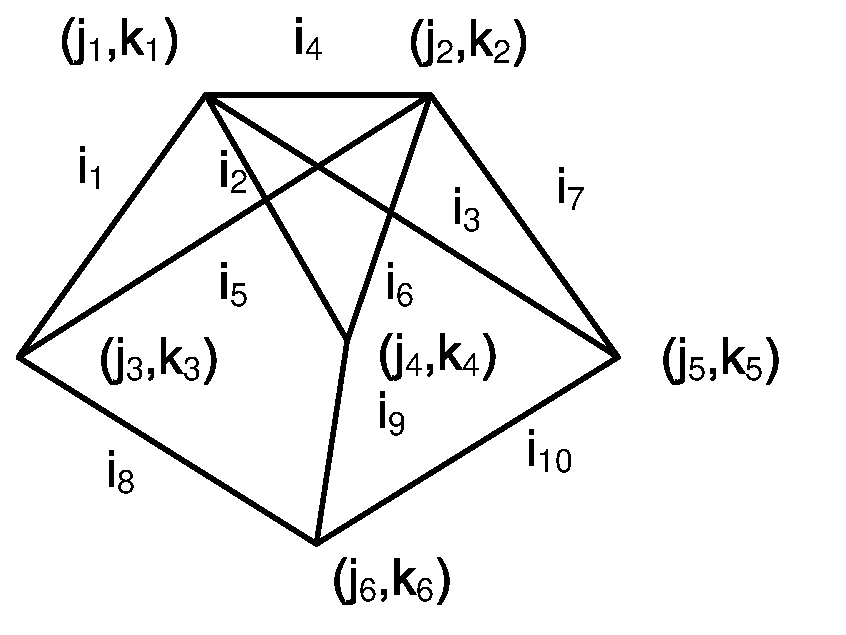
\includegraphics[width=3.2in,height=1.9in]{Drawing641_1.eps}
\caption{Depiction of the first candidate (6,4) set}\label{fig64a}
\end{figure}
\begin{figure}\center
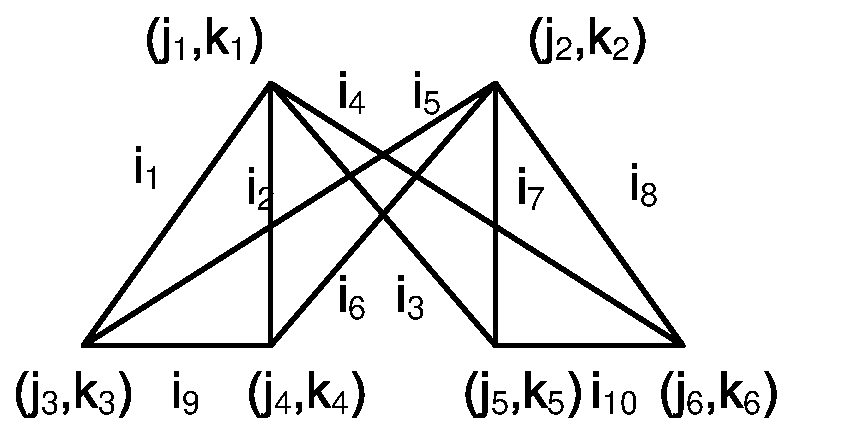
\includegraphics[width=3.2in,height=1.6in]{Drawing643_1.eps}
\caption{Depiction of the second candidate (6,4)
set}\label{fig64b}
\end{figure}
\begin{figure}
\center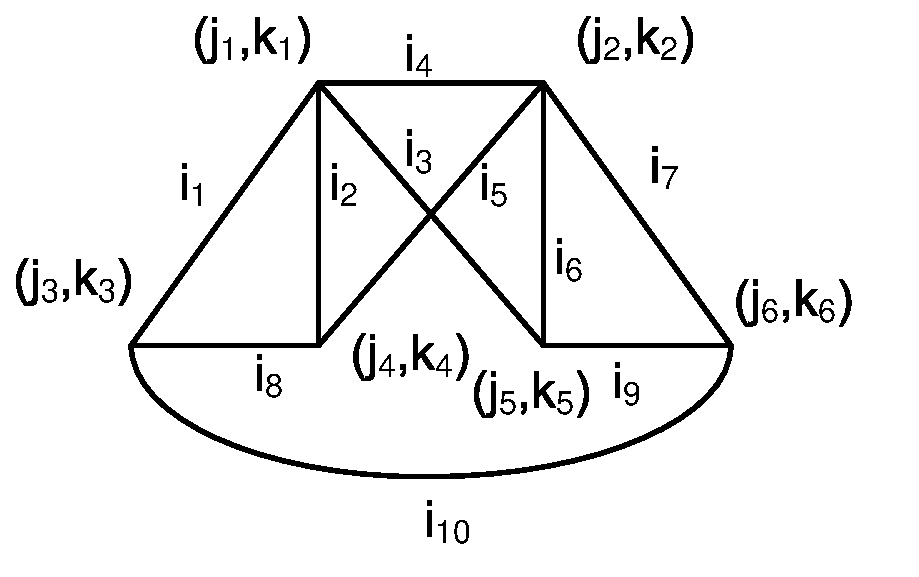
\includegraphics[width=3.2in,height=1.65in]{Drawing642_2.eps}
\caption{Depiction of the third candidate (6,4) set} \label{fig64c}
\end{figure}
We will first show that all satisfied checks neighboring bit nodes
in one such absorbing set must have degree 2. Note that there
cannot be a degree-6 check with respect to the bits in the
absorbing set as then some of these bits would have to share
another satisfied check which is not possible by the girth
condition. Suppose that there exists a check node of degree 4 with
respect to a $(6,4)$ absorbing set. Let $t_1, t_2,t_3,t_4$ be the
bit nodes in the absorbing set participating in degree-4 check
node, and let $t_5$ and $t_6$ be the remaining two bit nodes in
the absorbing set. By the girth condition there can be at most one
degree-4 check incident to the bit nodes in the absorbing set. If
at least one of $t_1, t_2,t_3,t_4$ had all check nodes satisfied,
it would be necessary that such a bit node shares another distinct
check node with some other bit node participating in the degree-4
check node, which is impossible by the girth constraint
\cite{fan}. Thus, all of $t_1, t_2,t_3,t_4$ are each connected to
3 satisfied and 1 unsatisfied check node. Then $t_5$ and $t_6$ are
each connected to 4 satisfied check nodes each of degree 2 with
respect to the bit nodes in the absorbing set. Since $t_1$ through
$t_4$ have 3 satisfied neighboring checks (one of which is a
degree-4 check by assumption), they each share a check with $t_5$
and with $t_6$. Therefore, $t_5$ and $t_6$ do not share a check.
Let $i_j$ for $1 \leq j \leq 4$ be the labels of the three check
nodes connecting $t_j$ and $t_5$. By the vertex consistency
condition at $t_5$, they are all different. By the vertex
consistency condition at each of $t_j$ for $1 \leq j \leq 4$, the
label of their shared degree-4 check node must be different from
all $i_j$ for $1 \leq j \leq 4$, which is impossible as there are
only 4 distinct labels available. Therefore, all satisfied check
nodes neighboring bit nodes in the absorbing set have degree 2.

%%%%%%%%%%%%%%%%%%%%%%%%%%%%%%%%%%%%%%%%%%%%%%%%%%%%%%%%%%%%%%%%%%%%
We consider a candidate (6,4) absorbing set in which three bit
nodes, call them $t_1,t_2,t_3$ connect to the same unsatisfied
check, and the remaining three bit nodes, call them $t_4,t_5,t_6$,
each have a distinct unsatisfied check. Since there are no cycles
of length 4, each of the $t_1,t_2,t_3$ shares a distinct satisfied
check with each of $t_4,t_5,t_6$.

We will show that for large enough prime $p$ such a configuration
is not possible.

Let the check incident to $t_1,t_2$, and $t_3$ have label $x$,
where $x \in \{0,1,2,3\}$. Using the vertex consistency condition,
we let $y$ be the label of the satisfied check incident to $t_1$
and $t_4$, $z$ be the label of the satisfied check incident to
$t_1$ and $t_5$, and $w$ be the label of the satisfied check
incident to $t_1$ and $t_6$, where $y,z,w \in \{0,1,2,3\}$ are
distinct and are different from $x$.

By propagating remaining edge labels while ensuring that the
vertex consistency is satisfied, we obtain that the labels of the
checks connecting $t_2$ with $t_4$, $t_5$  and $t_6$,
respectively, are $z$, $w$ and $y$ and the labels of the checks
connecting $t_3$ with $t_4$, $t_5$  and $t_6$, respectively, are
$w$, $y$ and $z$.

Let $(j_l,k_l)$ for $1 \leq l \leq 6$ be the labels of the bit
nodes $t_l$.

Using the parity check consistency we write one equation for each
pair of the bit nodes in the absorbing set that share a satisfied
check as follows:
\begin{equation}\label{eq1}\begin{array}{cccc}
k_1+yj_1 \equiv k_4+yj_4 \mod p,\\
k_1+zj_1 \equiv k_5+zj_5 \mod p,\\
k_1+wj_1 \equiv k_6+wj_6 \mod p,\\
k_2+zj_2 \equiv k_4+zj_4 \mod p,\\
k_2+wj_2 \equiv k_5+wj_5 \mod p,\\
k_2+yj_2 \equiv k_6+yj_6 \mod p,\\
k_3+wj_3 \equiv k_4+wj_4 \mod p,\\
k_3+yj_3 \equiv k_5+yj_5 \mod p,\\
k_3+zj_3 \equiv k_6+zj_6 \mod p~.
\end{array}\end{equation}

In addition we may also write
\begin{equation}\label{eq2}
k_1+xj_1 \equiv k_2+xj_2 \equiv k_3+xj_3 \mod p,
\end{equation}
since the bit nodes $(j_1,k_1)$, $(j_2,k_2)$ and $(j_3,k_3)$, all
participate in the same (unsatisfied) check with label $x$.

Since $x,y,z,w \in \{0,1,2,3\}$ and are distinct we now consider
different numerical assignments of these labels. In particular, it
is sufficient to consider $x=0$ and $y=0$, since by the symmetry
of the configuration both $z=0$ and $w=0$ reduce to the $y=0$
case.

1. Case $x=0$

Equation \eqref{eq2} reduces to
\begin{equation}
k_1 = k_2 = k_3,
\end{equation}
which combined with \eqref{eq1} gives
\begin{equation}\begin{array}{cccc}
k_1-k_4 \equiv y(j_4-j_1) \equiv z(j_4-j_2) \equiv w(j_4-j_3) \mod
p\\
k_1-k_5 \equiv z(j_5-j_1) \equiv w(j_5-j_2) \equiv y(j_5-j_3) \mod
p\\
k_1-k_6 \equiv w(j_6-j_1) \equiv y(j_6-j_2) \equiv z(j_6-j_3) \mod
p
\end{array}
\end{equation}

Since $y,z,w$ do not have any non trivial factors, we may let
$yzwt \equiv k_1-k_4 \mod p$, $yzwv \equiv k_1-k_5 \mod p$ and
$yzws \equiv k_1-k_6 \mod p$ for some integers $t,v$ and $s$.

Using the identity
\begin{equation}
j_5-j_4 = (j_5-j_1)-(j_4-j_1) = (j_5-j_2)-(j_4-j_2)
=(j_5-j_3)-(j_4-j_3)
\end{equation}
we obtain (using $(j_5-j_1) \equiv ywv \mod p,(j_4-j_1) \equiv zwt
\mod p$, and so on),
\begin{equation}
ywv-zwt \equiv yzv - ywt \equiv zwv -yzt \mod p~.
\end{equation}
The last expression implies
\begin{equation}\label{eq3}
y^2(w-z)^2 \equiv wz(z-y)(y-w) \mod p~.
\end{equation}

Likewise, using the identity
\begin{equation}
j_6-j_5 = (j_6-j_1)-(j_5-j_1) = (j_6-j_2)-(j_5-j_2)
=(j_6-j_3)-(j_5-j_3)
\end{equation}
we obtain
\begin{equation}
yzs-ywv \equiv zws-yzv \equiv yws-zwv \mod p~,
\end{equation}
and from it
\begin{equation}\label{eq4}
z^2(y-w)^2 \equiv yw(z-y)(w-z) \mod p~.
\end{equation}

Using the identity
\begin{equation}
j_6-j_4 = (j_6-j_1)-(j_4-j_1) = (j_6-j_2)-(j_4-j_2)
=(j_6-j_3)-(j_4-j_3)
\end{equation}
we obtain
\begin{equation}
yzs-zwt \equiv zws-ywt \equiv yws-yzt \mod p~,
\end{equation}
and from it
\begin{equation}\label{eq5}
w^2(z-y)^2 \equiv zy(w-z)(y-w) \mod p~.
\end{equation}

Since $\{y,z,w\}=\{1,2,3\}$, the equations \eqref{eq3},
\eqref{eq4} and \eqref{eq5} hold only for prime $p=13$.

 2. Case $y=0$

In this case equation \eqref{eq2} implies
\begin{equation}\begin{array}{ccc}
k_1 = k_4 \\
k_3 = k_5 \\
k_2 = k_6~.
\end{array}\end{equation}

Combined with \eqref{eq1}, we further obtain
\begin{equation}\begin{array}{ccc}
k_1 -k_3 \equiv z(j_5-j_1) \equiv w(j_3-j_4) \equiv x(j_3-j_1)
\mod p\\
k_1 -k_2 \equiv w(j_6-j_1) \equiv z(j_2-j_4) \equiv x(j_2-j_1)
\mod p\\
k_2 -k_3 \equiv w(j_5-j_2) \equiv z(j_3-j_6) \equiv x(j_3-j_2)
\mod p~.
\end{array}\end{equation}

We let $xzwt \equiv k_1-k_3 \mod p$, $xzwv \equiv k_1-k_2 \mod p$,
and $xzws \equiv k_2-k_3 \mod p$, for some integers $t,v$ and $s$.

From $k_1-k_3=k_1-k_2+k_2-k_3$, we have
\begin{equation}\label{eq6}
t \equiv v+s \mod p.
\end{equation}

From $j_6-j_1=-(j_3-j_6)+(j_3-j_1)$ we get
\begin{equation}\label{eq7}
zxv \equiv -wxs+zwt \mod p.
\end{equation}

Likewise, from $j_5-j_1=(j_5-j_2)+(j_2-j_1)$ we get
\begin{equation}\label{eq8}
xwt \equiv xzs+zwv \mod p,
\end{equation}
and from $j_3-j_4=(j_3-j_2)+(j_2-j_4)$ we get
\begin{equation}\label{eq9}
xzt \equiv zws+xwv \mod p~.
\end{equation}

From \eqref{eq6} and \eqref{eq7} by equating the expressions for
$zwt$ we obtain
\begin{equation}\label{eq10}
zv(x-w) \equiv ws(z-x) \mod p.
\end{equation}
Likewise, from \eqref{eq6} and \eqref{eq8} by equating the
expressions for $xwt$ we obtain
\begin{equation}\label{eq11}
wv(z-x) \equiv xs(w-z) \mod p, \end{equation} and from \eqref{eq6}
and \eqref{eq9} by equating the expressions for $xzt$ we obtain
\begin{equation}\label{eq12}
xv(z-w) \equiv zs(w-x) \mod p, \end{equation}

From \eqref{eq10}, \eqref{eq11} and \eqref{eq12}, it follows that
\begin{equation}
\begin{array}{ccc}
w^2(z-x)^2 \equiv xz(w-z)(x-w) \mod p,\\
-z^2(x-w)^2 \equiv xw(z-x)(z-w) \mod p,\\
-x^2(w-z)^2 \equiv wz(w-x)(z-x) \mod p~,
\end{array}\end{equation}
which are the same as conditions \eqref{eq3}, \eqref{eq4} and
\eqref{eq5} previously derived for the $x=0$ case.

Therefore, for prime $p, p>13$ the candidate configuration does
not exist.
 %%%%%%%%%%%%%%%%%
 %%%  NEW STUFF 10/8 %%%%%%%%%%
%XXXX figure plus analysis

By separately considering the cases when the two bit nodes that
have all neighboring checks satisfied have a satisfied check in
common, and the cases when they do not, one can show that there
are 3 possible non isomorphic configurations, as shown in
Figure~\ref{fig64a},~\ref{fig64b}, and~\ref{fig64c}. By ensuring
the vertex consistency, it further follows that for each
configuration there are 8 distinct edge labellings (as we show
below).

Let us consider the topmost configuration first. The other two
configurations are analyzed subsequently.

\textbf{I. Candidate (6,4) configuration, given in Figure
~\ref{fig64a}.}

\comment{As before, we establish a congruential constraint for
each triplet consisting of an edge and its endpoints given in
Figure~\ref{fig64a}. The set of constraints consisting of 10 such
equations, one for each edge, is
\begin{eqnarray*}
k_1+i_1j_1 &\equiv& k_3+i_1j_3 \mod p, \\
k_1+i_2j_1 &\equiv& k_4+i_2j_4 \mod p,\\
k_1+i_3j_1 &\equiv& k_5+i_3j_5 \mod p, \\
k_1+i_4j_1 &\equiv& k_2+i_4j_2 \mod p, \\
k_2+i_5j_2 &\equiv& k_3+i_5j_3 \mod p, \\
k_2+i_6j_2 &\equiv& k_4+i_6j_4 \mod p, \\
k_2+i_7j_2 &\equiv& k_5+i_7j_5 \mod p, \\
k_3+i_8j_3 &\equiv& k_6+i_8j_6 \mod p, \\
k_4+i_9j_4 &\equiv& k_6+i_9j_6 \mod p,\text{and} \\
k_5+i_{10}j_5 &\equiv& k_6+i_{10}j_6 \mod p.
\end{eqnarray*}
}

We first determine all possible edge labellings. For convenience,
we assign $(i_1,i_2,i_3,i_4)$ $\asn$ $(x,y,z,w)$, where $x,y,z,w
\in \{0,1,2,3 \}$ and distinct by the vertex consistency condition
at $(j_1,k_1)$. Then, by imposing the vertex consistency
conditions at remaining vertices, the possible assignments for the
remaining edge labels are as follows
\begin{equation}\label{tuples}\begin{array}{cccccc} (i_5,i_6,i_7,i_8,i_9,i_{10}) \in
 \{(y,z,x,z,x,y), (z,x,y,y,z,x),  \\
 (y,z,x,z,w,y),
(y,z,x,w,x,y),  (y,z,x,z,x,w),\\(z,x,y,y,z,w)
(z,x,y,y,w,x),(z,x,y,w,z,x) \}. \end{array}\end{equation}

We first observe that the assignments
$(i_1,i_2,i_3,i_4,i_5,i_6,i_7,i_8,i_9,i_{10})$
=$(x,y,z,w,y,z,x,z,x,y)$ and
$(i_1,i_2,i_3,i_4,i_5,i_6,i_7,i_8,i_9,i_{10})$
=$(x,y,z,w,z,x,y,y,z,x)$ are in fact symmetric (exchange $y$ and
$z$) and is thus sufficient to analyze only one of them.

Likewise, by appealing to symmetry and after appropriate
renamings, the remaining six assignments also represent the same
labelled configuration. In particular, third and sixth assignments
in~\eqref{tuples} are symmetric,  as are fourth and seventh, and
as are fifth and eighth assignments. Fourth assignment follows
from the third by exchanging the labels $x$ and $y$, and the fifth
assignment follows from the third by exchanging the labels $x$ and
$z$. It is thus sufficient to consider only
$(i_1,i_2,i_3,i_4,i_5,i_6,i_7,i_8,i_9,i_{10})$=
$(x,y,z,w,y,z,x,z,x,y)$ or $(x,y,z,w,y,z,x,z,w,y)$.

\underline{1. Case $(i_1,i_2,i_3,i_4,i_5,i_6,i_7,i_8,i_9,i_{10})$=
$(x,y,z,w,y,z,x,z,x,y)$}

By applying the parity check consistency for each edge and its end
points in Figure~\ref{fig64a} we obtain
\begin{equation}\label{con64a}\begin{array}{cccc}
k_1+xj_1 &\equiv& k_3+xj_3 \mod p, \\
k_1+yj_1 &\equiv& k_4+yj_4 \mod p,\\
k_1+zj_1 &\equiv& k_5+zj_5 \mod p, \\
k_1+wj_1 &\equiv& k_2+wj_2 \mod p, \\
k_2+yj_2 &\equiv& k_3+yj_3 \mod p, \\
k_2+zj_2 &\equiv& k_4+zj_4 \mod p, \\
k_2+xj_2 &\equiv& k_5+xj_5 \mod p, \\
k_3+zj_3 &\equiv& k_6+zj_6 \mod p, \\
k_4+xj_4 &\equiv& k_6+xj_6 \mod p,\text{and} \\
k_5+yj_5 &\equiv& k_6+yj_6 \mod p.
\end{array}\end{equation}

Using the cycle consistency conditions for each of the five cycles
in Figure~\ref{fig64a} we also write
\begin{equation}\label{con64b}\begin{array}{cccc}
w(j_2-j_1)+y(j_3-j_2)+x(j_1-j_3) \equiv 0 \mod p\\
w(j_2-j_1)+z(j_4-j_2)+y(j_1-j_4) \equiv 0 \mod p\\
w(j_2-j_1)+x(j_5-j_2)+z(j_1-j_5) \equiv 0 \mod p\\
y(j_4-j_1)+x(j_6-j_4)+z(j_3-j_6)+x(j_1-j_3) \equiv 0 \mod p\\
x(j_5-j_2)+y(j_6-j_5)+x(j_4-j_6)+z(j_2-j_4) \equiv 0 \mod p.
\end{array}\end{equation}


We will use the relationships in~\eqref{con64b} to express $j_3$
through $j_6$ in terms of $j_1$ and $(j_2-j_1)$, and then in turn
use~\eqref{con64a} to express $k_2 $ through $k_6$ in terms of
$k_1$, $j_1$ and $(j_2-j_1)$.


 By symmetry of the
configuration (see Figure~\ref{fig64a}), for the current labelling
it is sufficient to consider $x=0$ and $w=0$. Specifically,
letting $y=0$ or $z=0$ reduces to the $x=0$ case.

We let $a \asn j_2-j_1$, $b \asn j_3-j_1$, $c \asn j_4-j_1$,
 $d \asn j_5-j_1$, and $e \asn j_6-j_1$.  Note that in particular
 by the edge consistency constraint, $a \neq 0$.

$\bullet$ Consider $x=0$.


The system in~\eqref{con64b} reduces to
 \begin{equation}\label{sys31aa}\begin{array}{ccccc}
 a(w-y)+by &\equiv 0 &\mod p\\
 a(z-w)+c(y-z)  &\equiv 0 &\mod p\\
 aw-dz &\equiv 0 &\mod p\\
 bz+yc-ze &\equiv 0 &\mod p\\
 az-cz-dy+ey &\equiv 0 &\mod p~.
 \end{array}
 \end{equation}

using~\eqref{sys31aa} we express $b$, $c$ , $d$ and $e$ in terms
of $a$. In particular, the last constraint in~\eqref{sys31aa} is
redundant as it follows from the previous four. Therefore, for $q
\asn j_1$ and $t \asn j_2-j_1$, all of the remaining values of
$j_3,j_4,j_5,j_6$ follow for each of the $3!=6$ choices of
$(y,z,w)$.

Using~\eqref{con64a} we further obtain
\begin{equation}\begin{array}{ccccc}
k_3 & \equiv& k_1 &\mod p\\
k_4 & \equiv& k_1-y(j_4-j_1) &\mod p\\
k_5 &\equiv& k_1-z(j_5-j_1) &\mod p\\
k_2 &\equiv& k_5 &\mod p\\
k_6 &\equiv& k_4 &\mod p. \end{array}\end{equation}

Therefore, we can express $k_2$ through $k_6$ in terms of $s \asn
k_2$, $q$ and $t$. The results for all choices of $(y,z,w)$ are
summarized in Table~\ref{table64}.
\hspace{-0.95in}\small{\hspace{-0.95in}\begin{table*}[ht]\vspace{-0.05in}\hspace{-0.95in}
\begin{tabular}{|c |c|c|c|c|c|c|c|c|c|c|c|c|c|}
  \hline
  % after \\: \hline or \cline{col1-col2} \cline{col3-col4} ...
  $y,z,w$ & $j_1$ & $j_2$ & $j_3$ & $j_4$ & $j_5$ & $j_6$ & $k_1$ & $k_2$ & $k_3$ & $k_4$ & $k_5$ & $k_6$ \\
  \hline
$3,2,1$&  $q$ & $q+t$ &  $q+2t/3$ &  $q-t$ &  $q+t/2$ & $q-5t/6$ &
$s$ & $s-t$ & $s$ & $s+3t$ & $s-t$ &
  $s+3t$\\
  $3,1,2$&$q$& $q+t$ &  $q+t/3$ &    $q+t/2$ &  $q+2t$ &   $q+11/6t$ & $s$ & $s-2t$ & $s$ & $s-3/2t$ & $s-2t$ &
  $s-3/2t$\\
 $2,3,1$& $q$ & $q+t$ &  $q+t/2$&    $q+2t$ &  $q+t/3$ &   $q+11t/6$ & $s$ & $s-t$ & $s$ & $s-4t$ & $s-t$ &
  $s-4t$\\
$2,1,3$&  $q$ & $q+t$ &  $q-t/2$ &  $q+2t$ &   $q+3t$ & $q+7t/2$ &
$s$ & $s-3t$ & $s$ & $s-4t$ & $s-3t$ &
  $s-8t$\\
 $1,2,3$& $q$ & $q+t$ &  $q-2t$ &    $q-t$ &    $q+3t/2$ &    $q-5t/2$ & $s$ & $s-3t$ & $s$ & $s+t$ & $s-3t$ &
  $s+t$\\
  $1,3,2$&$q$ & $q+t$ &  $q-t$ &    $q+1/2t$ &  $q+2t/3$ &   $q-5/6t$ & $s$ & $s-2t$ & $s$ & $s-1/2t$ & $s-2t$ &
  $s-1/2t$\\
  \hline
\end{tabular}
\caption{ Several solution sets for the (6,4)
configuration.}\label{table64}
\end{table*}} \normalsize

\comment{[        q,      q+t,  q+2/3*t,      q-t,  q+1/2*t,
q-5/6*t, s, s-t,        s,    s+3*t,      s-t,    s+3*t]

[ q, q+t, q+1/3*t,  q+1/2*t,    q+2*t, q+11/6*t,        s,
s-2*t, s, s-3/2*t,    s-2*t,  s-3/2*t]

[        q,      q+t,  q+1/2*t, q+2*t,  q+1/3*t, q+11/6*t,
s,      s-t,        s,    s-4*t, s-t,    s-4*t]

[        q, q+t,  q-1/2*t,    q+2*t,    q+3*t, q+7/2*t,        s,
s-3*t, s,    s-4*t,    s-3*t, s-4*t]

[        q,      q+t, q-2*t, q-t,  q+3/2*t, q-5/2*t, s, s-3*t,
s,      s+t, s-3*t, s+t]

[        q, q+t, q-t, q+1/2*t,  q+2/3*t, q-5/6*t, s, s-2*t, s,
s-1/2*t, s-2*t, s-1/2*t]}
%file temp20.m

Furthermore, under the current configuration, the bit nodes in one
such $(6,4)$ absorbing set that have 3 satisfied and 1 unsatisfied
check, all have unsatisfied checks in the row group labelled $w$.
By the edge consistency condition, no bit node can connect to more
than one such check. Therefore, this configuration is in fact a
$(6,4)$ fully absorbing set.

The (absolute) indices of columns that correspond to the bit nodes
in the absorbing set are $k_i+pj_i$ for $1 \leq i \leq 6$ and the
indices of rows that correspond to the unsatisfied check nodes in
the absorbing set are $(k_i+j_iw) \mod p+ wp$, for $3\leq i \leq
6$. In particular, the solution set in row 1 holds for all $p > 5$
and $t$ a multiple of $6$.

%%%% comment starts here
\comment{The system~\eqref{con64a} reduces to
\begin{equation}\begin{array}{ccccccccc}
k_1-k_3 &\equiv& 0 & {}& {}&{}&{}&\mod p
\\
k_2-k_5 &\equiv& 0 & {}& {}&{}&{}&\mod p
\\
k_4-k_6 &\equiv& 0 & {}& {}&{}&{}&\mod p
\\
k_1-k_4 &\equiv& y(j_4-j_1) &\equiv& z(j_6-j_3) &{}& {}&\mod p\\
k_2-k_4 &\equiv& z(j_4-j_2) & \equiv& y(j_6-j_5) &{} & {}&\mod p\\
 k_1-k_2 &\equiv& z(j_5-j_1) & \equiv& w(j_2-j_1) &\equiv& y(j_2-j_3)& \mod p~.
\end{array}\end{equation}


For convenience we let
\begin{equation}\label{eq29}\begin{array}{cccc}
k_1-k_4 &\equiv yzv &\mod p \\
k_1-k_2 &\equiv yzwt &\mod p\\
k_2-k_4 &\equiv yzs &\mod p,
\end{array}\end{equation}
for appropriately chosen integers $v,t$ and $s$.

From~\eqref{con64a} and~\eqref{eq29} we obtain
\begin{equation}\label{eq29a}\begin{array}{cccc}
\end{array}\end{equation}

We may express By fixing the values of $j_1$ and $t$, the rest of
$j_2$ through $j_6$ as well as $u$ and $s$ follow uniquely for
chosen $y,z$ and $w$ since based on the above we may write
\begin{equation}\label{eq30}
\left[ \begin{array}{ccccccc} 0 & 0 & 1 & 0 & 0 & -z &0\\
0 & 0 & 0 & 1 & 0 & 0 &0\\
1 & 0 & 0 & 0 & 0 & 0 &0\\
1 & -1 & 0 & 0 & 0 & 0 &0\\
-1 & 0 & 1 & 0 & 0 & 0 &-y\\
0 & -1 & 0 & 0 & 1 & -y &0\\
0 & 0 & 0 & -1 & 1 & 0 & -z
\end{array}\right] \left[\begin{array}{c}
j_2\\j_3\\j_4\\j_5\\j_6\\v\\s\end{array}\right] \equiv
\left[\begin{array}{c}j_1\\j_1+ywt\\j_1+yzt\\zwt\\0\\0\\0\end{array}\right]
\mod p~.
\end{equation}

Note that neither the vector multiplying the matrix nor the vector
on the right hand side cannot be an all-zeros vector as otherwise
the consistency conditions would be violated.

By inverting the matrix above, and using the relationships of these
variables with $k_1$ through $k_6$ we obtain the system of solutions
listed in Figure~\ref{table64}. As indicated, each row in the table
corresponds to a different numerical assignment of $y$, $z$ and $w$
(recall that $x=0$ for all six cases). In the table $q$, $t$ and $s$
are arbitrary residues $\mod p$ and the entries should be
interpreted $\mod p$. Note that we have thus established the
existence of $(6,4)$ absorbing sets. Moreover, the solutions for $s$
and $v$ obtained from \eqref{eq30} agree with \eqref{eq29}.

Furthermore, under the current configuration, the bit nodes in one
such $(6,4)$ absorbing set that have 3 satisfied and 1 unsatisfied
check, all have unsatisfied checks in the row group labelled $w$. By
the edge consistency condition, no bit node can connect to more than
one such check. Therefore, this configuration is in fact a $(6,4)$
fully absorbing set.

The (absolute) indices of columns that correspond to the bit nodes
in the absorbing set are $k_i+pj_i$ for $1 \leq i \leq 6$ and the
indices of rows that correspond to the unsatisfied check nodes in
the absorbing set are $(k_i+j_iw) \mod p+ wp$, for $3\leq i \leq 6$.
In particular, the solution set in row 1 holds for all $p > 5$.

\hspace{-0.95in}\small{\hspace{-0.95in}\begin{table*}[ht]\vspace{-0.05in}\hspace{-0.95in}
\begin{tabular}{|c |c|c|c|c|c|c|c|c|c|c|c|c|c|}
  \hline
  % after \\: \hline or \cline{col1-col2} \cline{col3-col4} ...
  $y,z,w$ & $j_1$ & $j_2$ & $j_3$ & $j_4$ & $j_5$ & $j_6$ & $k_1$ & $k_2$ & $k_3$ & $k_4$ & $k_5$ & $k_6$ \\
  \hline
$3,2,1$&  $q$ & $q+6t$ &  $q+4t$ &  $q-6t$ &  $q+3t$ & $q-5t$ & $s$
& $s-6t$ & $s$ & $s+18t$ & $s-6t$ &
  $s+18t$\\
  $3,1,2$&$q$& $q+3t$ &  $q+t$ &    $q+3/2t$ &  $q+6t$ &   $q+11/2t$ & $s$ & $s-6t$ & $s$ & $s-9/2t$ & $s-6t$ &
  $s-9/2t$\\
 $2,3,1$& $q$ & $q+6t$ &  $q+3t$&    $q+12t$ &  $q+2t$ &   $q+11t$ & $s$ & $s-6t$ & $s$ & $s-24t$ & $s-6t$ &
  $s-24$\\
$2,1,3$&  $q$ & $q+2t$ &  $q-t$ &  $q+4t$ &   $q+6t$ &    $q+7t$ &
$s$ & $s-6t$ & $s$ & $s-8t$ & $s-6t$ &
  $s-8t$\\
 $1,2,3$& $q$ & $q+2t$ &  $q-4t$ &    $q-2t$ &    $q+3t$ &    $q-5t$ & $s$ & $s-6t$ & $s$ & $s+2t$ & $s-6t$ &
  $s+2t$\\
  $1,3,2$&$q$ & $q+3t$ &  $q-3t$ &    $q+3/2t$ &  $q+2t$ &   $q-5/2t$ & $s$ & $s-6t$ & $s$ & $s-3/2t$ & $s-6t$ &
  $s-3/2t$\\
  \hline
\end{tabular}
\caption{ Several solution sets for the (6,4)
configuration.}\label{table64}
\end{table*}}
\normalsize }
%\textbf{comment on s and u being consistent} \textbf{comment on
%singularity}
%%%%% comment ends here

We complete the analysis of this label assignment by considering
$w=0$.

$\bullet$ Consider $w=0$.



In this case the system in~\eqref{con64b} reduces to:
 \begin{equation}\label{sys31a}\begin{array}{ccccc}
 ay+b(x-y) &\equiv 0 &\mod p\\
 az+c(y-z)  &\equiv 0 &\mod p\\
 ax+d(z-x) &\equiv 0 &\mod p\\
 b(z-x)+c(y-x)+e(x-z) &\equiv 0 &\mod p\\
 a(z-x)+c(x-z)+d(x-y)+e(y-x) &\equiv 0 &\mod p~.
 \end{array}
 \end{equation}


Note that the last relation follows from the previous four. We
again express $b$, $c$ $d$ and $e$ in terms of $a$, so that by
setting $j_1 \asn q$ and $a \asn t$, all of $j_2$ through $j_6$
follow as a function of $q$ and $t$. Then, by letting $k_1 \asn
s$, the remaining $k_2$ through $k_6$ follow from $q,t$ and $s$,
from~\eqref{con64a}. The solution set for various numerical
assignments of $(x,y,z)$ is given in Table~\ref{table641}.
\hspace{-0.95in}\small{\hspace{-0.95in}\begin{table*}[ht]\vspace{-0.05in}\hspace{-0.95in}
\begin{tabular}{|c |c|c|c|c|c|c|c|c|c|c|c|c|c|}
  \hline
  % after \\: \hline or \cline{col1-col2} \cline{col3-col4} ...
  $y,z,w$ & $j_1$ & $j_2$ & $j_3$ & $j_4$ & $j_5$ & $j_6$ & $k_1$ & $k_2$ & $k_3$ & $k_4$ & $k_5$ & $k_6$ \\
  \hline
    $3,2,1$ & $q$ &$q+t$ & $q-2t$ & $q-t$& $q+3/2t$ &$q-5t/2$ & $s$ &$s$ &   $s+6t$ & $s+2t$ & $s-3/2t$ &
    $s+13/2t$\\
     $3,1,2$ & $q$ &$q+t$ & $q-t/2$ & $q+2t$& $q+3t$ &$q+7t/2$ & $s$ &$s$ &   $s+3t/2$ & $s-2t$ & $s-6t$ &
    $s-13/2t$\\
     $2,3,1$ & $q$ &$q+t$ & $q+3t$ & $q-t/2$& $q+2t$ &$q+7t/2$ & $s$ &$s$ &   $s-6t$ & $s+3t/2$ & $s-2t$ &
    $s-13/2t$\\
     $2,1,3$ & $q$ &$q+t$ & $q-t$ & $q+3t/2$& $q-2t$ &$q-5t/2$ & $s$ &$s$ &   $s+2t$ & $s-3t/2$ & $s+6t$ &
    $s+13/2t$\\
     $1,2,3$ & $q$ &$q+t$ & $q+2t$ & $q+3t$& $q-t/2$ &$q+7t/2$ & $s$ &$s$ &   $s-2t$ & $s-6t$ & $s+3/2t$ &
    $s-13/2t$\\
     $1,3,2$ & $q$ &$q+t$ & $q+3t/2$ & $q-2t$& $q-t$ &$q-5t/2$ & $s$ &$s$ &   $s-3t/2$ & $s+6t$ & $s+2t$ &
    $s+13/2t$\\
  \hline
\end{tabular}
\caption{ Several solution sets for the (6,4)
configuration.}\label{table641}
\end{table*}}
\normalsize %\textbf{comment on fully absorbing sets}
%%%% this is in temp16.m
 \comment{    [        q,      q+t, q-2*t,
q-t, q+3/2*t, q-5/2*t, s,        s,    s+6*t,    s+2*t, s-3/2*t,
s+13/2*t] [ q, q+t,  q-1/2*t,    q+2*t,    q+3*t, q+7/2*t, s, s,
s+3/2*t, s-2*t,    s-6*t, s-13/2*t] [        q, q+t,    q+3*t,
q-1/2*t, q+2*t,  q+7/2*t,        s,        s, s-6*t,  s+3/2*t,
s-2*t, s-13/2*t] [        q,      q+t, q-t, q+3/2*t,    q-2*t,
q-5/2*t, s,        s,    s+2*t, s-3/2*t, s+6*t, s+13/2*t] [ q,
q+t,    q+2*t, q+3*t,  q-1/2*t, q+7/2*t, s, s, s-2*t, s-6*t,
s+3/2*t, s-13/2*t] [        q, q+t, q+3/2*t, q-2*t, q-t, q-5/2*t,
s,        s,  s-3/2*t, s+6*t, s+2*t, s+13/2*t] }


Recall that we are still considering the case where the unsatisfied
checks all belong in the row group labelled $w$. By the edge
consistency condition, no bit node can connect to more than one such
check. Therefore, this configuration is also in fact a $(6,4)$ fully
absorbing set.

The (absolute) indices of columns that correspond to the bit nodes
in the absorbing set are $k_i+pj_i$ for $1 \leq i \leq 6$ and the
indices of rows that correspond to the unsatisfied check nodes in
the absorbing set are $(k_i+j_iw) \mod p+ wp$, for $3\leq i \leq 6$.
In particular, the solution set in row 1 of the table in
Figure~\ref{table641}holds for all $p
> 5$ and $t$ even.


 The remaining labelled configuration of Figure~\ref{fig64a} to be considered is
$(i_1,i_2,i_3,i_4,i_5,i_6,i_7,i_8,i_9,i_{10})$ =
$(x,y,z,w,y,z,x,z,w,y)$.

We let $a \asn j_2-j_1$, $b \asn j_3-j_1$, $c \asn j_4-j_1$,
 $d \asn j_5-j_1$, and $e \asn j_6-j_1$.  Note that in particular
 by the edge consistency constraint, $a \neq 0$.

Based on the cycles consistency condition for the five cycles in
Figure~\ref{fig64a} we establish
 \begin{equation}\label{sys31}\begin{array}{cccc}
 a(w-y)+b(y-x) &\equiv 0 &\mod p\\
 a(w-z)+c(z-y) &\equiv 0 &\mod p\\
 a(w-x)+d(x-z) &\equiv 0 &\mod p\\
 c(y-w)+b(z-x)+e(w-z) &\equiv 0 &\mod p\\
 d(x-y)+a(z-x)+c(w-z)+e(y-w)&\equiv 0 &\mod p~.
 \end{array}
 \end{equation}



By expressing $b$, $c$ and $d$ in terms of $a$, from this system
we obtain
\begin{eqnarray}\label{sys32a}
a\left(\frac{(y-w)(w-z)}{y-z}+\frac{(z-x)(w-y)}{x-y} \right)+e(w-z)p &\equiv 0 &\mod p\\
\label{sys32b}a\left(\frac{(x-y)(w-x)}{z-x}+(z-x)+\frac{(w-z)^2}{y-z)}
\right)+e(y-w)&\equiv 0 &\mod p,
\end{eqnarray}
where $\{x,y,z,w\} =\{0,1,2,3\}$ and are distinct. For all $4!=24$
distinct ways of assigning numerical values to $x,y,z$ and $w$, the
system \eqref{sys32a}--\eqref{sys32b} produces the unique solution
$a=0$, $e=0$, provided that $p>3$. Since $a\neq 0$ by the edge
consistency condition, we conclude that this configuration is not
possible.

\comment{temp5.m and temp6.m and temp7.m which are superseded by
temp15.m} \comment{temp14.m and temp15.m} %\textbf{put this first}

We now consider the second candidate (6,4) configuration.

\textbf{II. Candidate (6,4) configuration, given in Figure
~\ref{fig64b}.}

We first determine all possible edge labellings. For convenience,
let $(i_1,i_2,i_3,i_4)$ $\asn$ $(x,y,z,w)$, where $x,y,z,w \in
\{0,1,2,3 \}$ and are distinct by the vertex consistency condition
at $(j_1,k_1)$. Then, by imposing the vertex consistency
conditions at remaining vertices, the assignments for the
remaining edge labels are given by the following set
\begin{equation}\label{tuples2}\begin{array}{cccc} (i_5,i_6,i_7,i_8,i_9,i_{10}) \in
 \{(y,x,w,z,z,x),(w,x,y,z,z,x),\\
 (y,x,w,z,z,y),(y,w,x,z,z,y),(y,x,w,z,w,x),\\(z,x,w,y,w,x),(y,z,w,x,w,y),(y,x,w,z,w,y)\}~.
\end{array}\end{equation}

Out of these 8 possible labelled configurations by appealing to
symmetry and label renaming it is sufficient to consider only 2 of
these as we now show. Note that the eighth labelling is the same
as the first labelling after we exchange $(j_3,k_3)$ and
$(j_4,k_4)$, $(j_5,k_5)$ and $(j_6,k_6)$, and labels $b$ with $a$
and $d$ with $c$. Likewise, the second labelling is the same as
the seventh labelling after we exchange $(j_3,k_3)$ and
$(j_4,k_4)$, $(j_5,k_5)$ and $(j_6,k_6)$, and labels $b$ with $a$
and $d$ with $c$. Sixth labelling is the same as the fourth
labelling after we exchange labels $c$ with $a$, $b$ with $d$, and
nodes $(j_1,k_1)$ with $(j_2,k_2)$, $(j_3,k_3)$ with $(j_4,k_4)$,
and $(j_5,k_5)$ with $(j_6,k_6)$, and take the mirror image of the
resulting configuration. Fifth labelling is the same as the third
after we exchange labels $c$ with $a$ and $b$ with $d$ and take
the mirror image of the whole configuration. Fourth (respectively
first) labelling is the same as the second (respectively third)
after we exchange $(j_3,k_3)$ and $(j_4,k_4)$ and labels $a$ and
$b$.

It is thus sufficient to consider only two different labellings,
namely $(i_1,i_2,i_3,i_4,i_5,i_6,i_7,i_8,i_9,i_{10})$=
$(x,y,z,w,y,x,w,z,z,y)$ (third labelling) and
$(i_1,i_2,i_3,i_4,i_5,i_6,i_7,i_8,i_9,i_{10})$ =
$(x,y,z,w,y,z,w,x,w,y)$ (seventh labelling).

For the first remaining cases by symmetry it is sufficient to
consider $x=0$ and $z=0$ as $w=0$ and $y=0$ reduce to the $x=0$
and $z=0$ case respectively. Likewise, for the second case it is
sufficient to consider $x=0$ and $y=0$, as $z=0$ and $w=0$ each
reduce to the $x=0$ and $y=0$ cases, respectively.

%Let us consider $(i_1,i_2,i_3,i_4,i_5,i_6,i_7,i_8,i_9,i_{10})$=
%$(x,y,z,w,y,x,w,z,z,y)$ first, with $x=0$.




We now consider $(i_1,i_2,i_3,i_4,i_5,i_6,i_7,i_8,i_9,i_{10})$=
$(x,y,z,w,y,x,w,z,z,y)$ first, starting with with $z=0$. \comment{
Consider $z=0$ XXXXXXXXXXX-6 THIS IS DONE. HAS ONE VALID
 SOLUTION. SEE TEMP2.M}

\underline{1. Case $(i_1,i_2,i_3,i_4,i_5,i_6,i_7,i_8,i_9,i_{10})$=
$(x,y,z,w,y,x,w,z,z,y)$}

$\bullet$ $z=0$.

 From Figure~\ref{fig64b} and under the current edge label
 assignment using the parity check consistency constraints we write
\begin{equation}\label{eq10a}\begin{array}{ccccc}
k_1 & \equiv &k_5 &\mod p\\
k_2 & \equiv &k_6 &\mod p\\
k_3 & \equiv &k_4 &\mod p\\
k_1+xj_1 & \equiv & k_3+xj_3 &\mod p\\
k_1+yj_1 & \equiv & k_4+yj_4 &\mod p\\
k_1+wj_1 & \equiv & k_6+wj_6 &\mod p\\
k_2+yj_2 & \equiv & k_3+yj_3 &\mod p\\
k_2+xj_2 & \equiv & k_4+xj_4 &\mod p\\
k_2+wj_2 & \equiv & k_5+wj_5 &\mod p\\
k_5+yj_5 & \equiv & k_6+yj_6 &\mod p~.
\end{array}\end{equation}

%%%%%%%%%%%%%%%%%%%%%%%%
%%%%%% NEW STUFF 10/8
%%%%%%%%%%%%%%%%%%%%%%%%
\comment{From \eqref{eq10a} we write
\begin{equation}\label{eq10b}\begin{array}{cccc}
k_2-k_3 &\equiv xyv &\mod p \\
k_1-k_2 &\equiv ywt &\mod p\\
k_1-k_3 &\equiv xys &\mod p,
\end{array}\end{equation}
for appropriately chosen integers $v,t$ and $s$. Note that by the
edge consistency condition all of $v,t$ and $s$ are non zero
residues $\mod p$.


We now express $j_2$ through $j_6$, $s$ and $v$ in terms of $j_1$
and $t$ based on \eqref{eq10a} and \eqref{eq10b}, as
\begin{equation}\label{eq10c}
\left[ \begin{array}{ccccccc} 0 & 0 & 0 & 0 & 1 & 0 &0\\
1 & 0 & 0 & -1 & 0 & 0 &0\\
0 & 0 & 0 & -1 & 1 & 0 &0\\
0 & 1 & 0 & 0 & 0 & -y &0\\
0 & 0 & 1 & 0 & 0 & -x &0\\
-1 & 1 & 0 & 0 & 0 & 0 &-x\\
-1 & 0 & 1 & 0 & 0 & 0 &-y
\end{array}\right] \left[\begin{array}{c}
j_2\\j_3\\j_4\\j_5\\j_6\\s\\v\end{array}\right] \equiv
\left[\begin{array}{c}j_1+yt\\yt\\wt\\j_1\\j_1\\0\\0\end{array}\right]
\mod p~.
\end{equation}

Note that neither the vector multiplying the matrix nor the vector
on the right hand side cannot be an all-zeros vector as otherwise
the consistency conditions would be violated.

In all $3!=6$ choices for $(x,y,w)$, the solution for $s$ and $v$
to \eqref{eq10c} expresses them as multiples of $t$. Since $wt
\equiv x(s-v) \mod p$ (write $k_1-k_2$ as $(k_1-k_3)-(k_2-k_3)$),
in all but one of these solutions, it then follows that $t \equiv
0 \mod p$ for $p>7$, which violates the edge consistency
condition. The remaining case (when $t$ is a non zero residue)
corresponds to $x=1$, $y=3$, and $w=2$ for which we establish the
solution set listed in Table~\ref{table64b} for $j_1=q$ and
$k_1=s$.} %%%%%%%%% END OF COMMENTED OUT STUFF 10/7
Let $a\asn j_2-j_1$, $b\asn j_3-j_1$, $c\asn j_4-j_1$, $d\asn
j_5-j_1$ and $e\asn j_6-j_1$. Using the cycle constraint for the
four cycles in Figure~\ref{fig64b} and under the current edge
labelling we have
\begin{equation}\label{eq1}\begin{array}{cccc}
xb+y(-c) &\equiv &0 \mod p, \\
y(b-a)+x(a-c) &\equiv &0 \mod p, \\
y(e-d) +w(-e) &\equiv &0 \mod p, \\
w(d-a)+y(e-d)&\equiv &0 \mod p .\end{array}\end{equation}

From the system \eqref{eq10a} we write
\begin{equation}\label{eq2}\begin{array}{lll}
k_1 -k_2 \equiv k_1-k_6 \equiv w(j_6-j_1) \equiv we &\mod p,\\
k_1-k_3 \equiv k_1 -k_4 \equiv y(j_4-j_1) \equiv yc &\mod p,\\
k_2 -k_3 \equiv y(j_3-j_2) \equiv y(b-a) &\mod p.
\end{array}\end{equation}
Using the identity $(k_1-k_2)=(k_1-k_3)-(k_2-k_3)$, and
\eqref{eq2} we obtain
\begin{equation}\label{eq3}
we \equiv y(c-b+a) \mod p.
\end{equation}

There are six possible assignments for $(x,y,w)$, as permutations
of the set $(1,2,3)$. In the remainder we will show that in fact
only $(x,y,w)=(1,3,2)$ gives rise to absorbing sets. In all other
cases, using \eqref{eq1} and \eqref{eq3}, we will reach a
contradiction.

From \eqref{eq1} we have
\begin{equation}\label{eq4}\begin{array}{ccc}
xb \equiv yc \mod p\\
yd \equiv (y-w)e \mod p.
\end{array}\end{equation}
We also have
\begin{equation}\label{eq5}\begin{array}{ccc}
xa -(y+x)c \equiv 0 \mod p\\
(2y-w)e \equiv ya \mod p,
\end{array}\end{equation}

where the top expression in \eqref{eq5} follows from substituting
top expression in \eqref{eq4} into the second expression of
\eqref{eq1} and the bottom expression in \eqref{eq5} follows from
substituting bottom expression in \eqref{eq4} into the fourth
expression of \eqref{eq1}.

For $(y,w,x)=(1,2,3)$, the bottom expression in \eqref{eq5} gives
\[
a \equiv 0 \mod p,\\
\]
which then implies
\[
c\equiv 0 \mod p,\\
\]
by the top expression in \eqref{eq5}. Since $c=j_4-j_1$, and
$(j_1,k_1)$ and $(j_4,k_4)$ share a check, $c$ must be non-zero,
implying a contradiction.

For $(y,w,x) \in \{ (1,3,2), (2,1,3), (2,3,1),(3,1,2)\}$ we
express $b,c,d,e$ in terms of $a$ using \eqref{eq4} and
\eqref{eq5}:

For $(y,w,x)=(1,3,2)$ we obtain \[b \equiv a/3 \mod p, c
\equiv2a/3 \mod p, d \equiv 2a \mod p, e \equiv -a \mod p.\]

For $(y,w,x)=(2,1,3)$ we obtain \[b \equiv 2a/5 \mod p, c \equiv
3a/5 \mod p, d \equiv a/3 \mod p, e \equiv 2a/3 \mod p.\]

For $(y,w,x)=(2,3,1)$ we obtain \[b \equiv 2a/3 \mod p, c \equiv
a/3 \mod p, d \equiv a \mod p, e \equiv 2a \mod p.\]

For $(y,w,x)=(3,1,2)$ we obtain \[b \equiv 3a/5 \mod p, c \equiv
2a/5 \mod p, d \equiv 2a/5 \mod p, e \equiv 3a/5 \mod p.\]

In all four cases, when $b,c$ and $e$ are substituted in
\eqref{eq3} it follows that $a \equiv 0 \mod p$ (we get $-3a
\equiv 4a/3 \mod p$, $2a/3 \equiv 12a/5 \mod p$, $6a \equiv 4a/3
\mod p$, and $3a/5 \equiv 12a/5 \mod p$, respectively). Since $b$
is a multiple of $a$ in all four cases, if $a \equiv 0 \mod p$,
then $b \equiv 0 \mod p$ as well. Since $b=j_3-j_1$ and nodes
$(j_1,k_1)$ and $(j_3,k_3)$ share a check, $b$ must be non-zero,
thus implying a contradiction.

For $(y,w,x)=(3,2,1)$ we obtain \[b \equiv 3a/4 \mod p, c \equiv
a/4 \mod p, d \equiv a/4 \mod p, e \equiv 3a/4 \mod p.\] When
$b,c$ and $e$ are substituted in \eqref{eq3}, we obtain the
identity $3a/2 \equiv 3a/2 \mod p$. Since $c \equiv d \mod p$, we
have that $j_4=j_5$ and since $b \equiv e \mod p$, we have that
$j_3=j_6$. Note that neither of these two conditions on $j$s
violates the edge consistency constraint since the respective bit
nodes do not share a check in Figure 12. Let $q=j_1$ and $t=j_4
-j_1$. Then $j_4=q+t$ and $j_5=q+t$. Since $b=3c$, and $b=j_3-j_1$
and $c=j_4-j_1$, we have that $j_3=q+3t$. Since $j_3=j_6$,
$j_6=q+3t$ as well. Likewise, since $a=4c$, and $a=j_2-j_1$ and
$c=j_4-j_1$, we have that $j_2=q+4t$. We have thus expressed all
of $j_1$ through $j_6$ in terms of $q$ and $t$. Now the system
\eqref{eq10a} reduces to
\begin{equation}\label{eq6}\begin{array}{ccc}
k_1 &\equiv& k_5 \mod p,\\
k_2 &\equiv& k_6 \mod p,\\
k_3 &\equiv& k_4 \mod p,\\
k_1 -k_3 &\equiv& 3t \mod p,\\
k_1 -k_2 &\equiv& 6t \mod p,\\
k_2 -k_3 &\equiv& -3t \mod p.\\
\end{array}\end{equation}

Thus, with $s=k_1$ and using \eqref{eq6} we can express all of
$k_1$ through $k_6$ in terms of $s$ and $t$. This solution set for
$j_1$ through $j_6$ and $k_1$ through $k_6$ is listed in Table
\ref{table64b}.

\hspace{-0.2in}\small{\hspace{-0.2in}\begin{table*}[ht]\vspace{-0.05in}\hspace{-0.2in}
\begin{tabular}{|c |c|c|c|c|c|c|c|c|c|c|c|c|c|}
  % after \\: \hline or \cline{col1-col2} \cline{col3-col4} ...
  \hline
  $x,y,w$ & $j_1$ & $j_2$ & $j_3$ & $j_4$ & $j_5$ & $j_6$ & $k_1$ & $k_2$ & $k_3$ & $k_4$ & $k_5$ & $k_6$ \\
  \hline
$1,3,2$&  $q$ & $q+4t$ &  $q+3t$ &  $q+t$ &  $q+t$ & $q+3t$ & $s$ &
$s-6t$ & $s-3t$ & $s-3t$ & $s$ &
  $s-6t$\\
  \hline
\end{tabular}
\caption{ A solution set for an (6,4) absorbing
set.}\label{table64b}
\end{table*}}
\normalsize

Note that the result in Table~\ref{table64b} establishes the
existence of a (6,4) absorbing set. We now discuss whether this
set is also a (6,4) fully absorbing set. Suppose there exists a
bit node $(j_7,k_7)$ outside this absorbing set that is incident
to some of the unsatisfied checks. By the vertex consistency
constraint, both $(j_3,k_3)$ and $(j_4,k_4)$ each have a
neighboring unsatisfied check whose label is $w$. These two checks
must be distinct by the girth condition. Likewise, both
$(j_5,k_5)$ and $(j_6,k_6)$ each have a neighboring unsatisfied
check whose label is $x$, and these are also distinct by the girth
condition. By the vertex consistency condition, the bit node
$(j_7,k_7)$ can then share at most 2 of these checks with the bit
nodes $(j_3,k_3)$ through $(j_4,k_4)$.

Suppose first that the bit node $(j_7,k_7)$ shares the check with
each of $(j_3,k_3)$ and $(j_5,k_5)$. From the cycles relating bit
nodes $(j_7,k_7)$, $(j_3,k_3)$, $(j_5,k_5)$, $(j_1,k_1)$, and
$(j_2,k_2)$, we obtain
\begin{eqnarray*}
x(j_7-j_5)+w(j_3-j_7)+x(j_1-j_3) &\equiv 0& \mod p\\
w(j_5-j_2)+x(j_7-j_5)+w(j_3-j_7)+y(j_2-j_3) &\equiv 0& \mod p~.
\end{eqnarray*}

For $(x,y,z,w)=(1,3,0,2)$ of present interest, we obtain that $j_7
\equiv q+2t \mod p$ using the result in Figure~\ref{fig64b}.

Since we further have
\begin{eqnarray*}
k_3+2j_3 &\equiv & k_7+2j_7 \mod p\\
k_5+j_5 & \equiv & k_7 +j_7 \mod p,
\end{eqnarray*}
it follows that $k_7 \equiv s-t \mod p$. Therefore by the existence
of this bit node $(j_7,k_7)$, the current (6,4) absorbing set is not
a (6,4) fully absorbing set.

%%% comment on other choices.

%%% in temp23.m using cycles

%%%%%%%%%%%%%%%%%%%%%%%%%%%%%%%%%%%%%%%%%%%%%%
%\textbf{comment on fully absorbing sets}

 We now consider
$(i_1,i_2,i_3,i_4,i_5,i_6,i_7,i_8,i_9,i_{10})$=
$(x,y,z,w,y,x,w,z,z,y)$ with $x=0$. \comment{Consider $x=0$
XXXXXXXXXXX=5 THIS IS DONE. VALID SOLS FOR 213 AND 231 IN TERMS OF
J1 AND K1}

$\bullet$ $x=0$

As before, using the parity check consistency constraints we
establish:
\begin{equation}\label{eq11c}\begin{array}{cccc}
k_1 & \equiv & k_3 \mod p\\
k_2 & \equiv & k_4 \mod p\\
k_1+yj_1 & \equiv & k_4+yj_4 \mod p\\
k_1+zj_1 & \equiv & k_5+zj_5 \mod p\\
k_1+wj_1 & \equiv & k_6+wj_6 \mod p\\
k_2+yj_2 & \equiv & k_3+yj_3 \mod p\\
k_2+wj_2 & \equiv & k_5+wj_5 \mod p\\
k_2+zj_2 & \equiv & k_6+zj_6 \mod p\\
k_3+zj_3 & \equiv & k_4+zj_4 \mod p\\
k_5+yj_5 & \equiv & k_6+yj_6 \mod p,~.
\end{array}\end{equation}

Let $a \asn j_2 -j_1$, $b \asn j_3 -j_1$, $c \asn j_4 -j_1$, $d
\asn j_5 -j_1$, and $e \asn j_6 -j_1$. Using the cycle constraints
for the four cycles in Figure~\ref{fig64b} we may also write
\begin{equation}\label{eq11d}\begin{array}{cccc}
z(c-b)+y(-c) &\equiv & 0 \mod p, \\
y(b-a)+z(c-b)&\equiv & 0 \mod p, \\
zd+y(e-d)+w(-e) &\equiv & 0 \mod p, \\
w(d-a)+y(e-d)+z(a-e) &\equiv & 0 \mod p~.
\end{array}\end{equation}


There are 6 possible assignments for $(y,z,w)$ as permutations of
the set $\{1,2,3\}$. We will show that in fact the only possible
assignment is $(y,z,w)=(2,1,3)$ (a contradiction will be reached
in all other cases).

Consider first the assignment $(y,z,w)=(1,2,3)$.
Using~\eqref{eq11d} we express $a$, $b$, $c$ and $d$ in terms of
$e$ so that
\begin{equation}\label{eq11e}\begin{array}{cccc}
a &\equiv & 3e \mod p, \\
b &\equiv & e \mod p, \\
c &\equiv & 2e \mod p, \\
d &\equiv & 2e \mod p~. \\
\end{array}\end{equation}

Note that since $c \equiv d \mod p$ and  $b \equiv e \mod p$ the
above implies that $j_4=j_5$ and $j_3=j_6$. Even though now some
vertices have the same $j$ components, the edge consistency
condition is not violated as $(j_4,k_4)$ and $(j_5,k_5)$ do not
share an edge, and neither do $(j_3,k_3)$ and $(j_6,k_6)$ (see
Figure~\ref{fig64b}).

From~\eqref{eq11c} and by substituting for $a$, $c$ and $d$ in
terms of $e$ using~\eqref{eq11e} we note that
\begin{equation}\label{eq11f}\begin{array}{cccc}
k_1-k_2 \equiv 1(2e) \mod p, \\
k_1-k_5 \equiv 2(2e) \mod p, \\
k_2-k_5 \equiv 3(2e-3e) \mod p~.
\end{array}\end{equation}

The system~\eqref{eq11f} implies that $e \equiv 0 \mod p$ for
$p>5$. Since $e=j_6-j_1$ and $(j_1,k_1)$ and $(j_6,k_6)$ do share
an edge, the condition $e \equiv 0 \mod p$ violates the edge
consistency constraint. We thus conclude that the current
numerical assignment for $(y,z,w)$ is not possible.

By expressing $a$, $b$, $c$ and $d$ in terms of $e$ as
in~\eqref{eq11e} and then using~\eqref{eq11c} to express the
differences $k_1-k_2$, $k_1-k_5$, and $k_2-k_5$ as
in~\eqref{eq11f} we conclude that $e \equiv 0 \mod p$ when
$(y,z,w)$ = $(1,3,2)$ and $p>5$ as well as $(y,z,w)$ = $(3,1,2)$
or $(3,2,1)$ and $p>7$.

Consider now the assignment $(y,z,w)=(2,3,1)$. Using~\eqref{eq11d}
it follows after substituting for $d$ in terms of $e$ in the last
expression that
\begin{eqnarray}
a \equiv 0 \mod p~.
\end{eqnarray}
By substituting for $b$ in terms of $c$ in the second expression
in~\eqref{eq11d} it also follows that
\begin{eqnarray}
3a \equiv 6c \mod p~.
\end{eqnarray}
Therefore $c \equiv 0 \mod p$, which violates the edge consistency
constraint for the edge connecting bit nodes $(j_1,k_1)$ and
$(j_4,k_4)$. The condition $a \equiv 0 \mod p$ by itself does not
yield a contradiction as the nodes $(j_1,k_1)$ and $(j_2,k_2)$ do
not have any edges in common.

Finally, we consider the assignment $(y,z,w)=(2,1,3)$. First, by
substituting for $d$ in terms of $e$ in the last expression that
\begin{eqnarray}
a \equiv 0 \mod p~.
\end{eqnarray}.
Therefore $j_1=j_2$. By substituting for $b$ in terms of $c$ in
the second expression in~\eqref{eq11d} we have that
\begin{eqnarray}
1a \equiv (2-2)c \mod p~,
\end{eqnarray}
which does not tell us anything about the actual value of $c$. We
express $b$, $c$ and $d$ in terms of $e$, again
using~\eqref{eq11d}, and obtain
\begin{equation}\label{eq11g}\begin{array}{cccc}
b &\equiv & -e \mod p, \\
c &\equiv & e \mod p, \\
d &\equiv & -e \mod p~. \\
\end{array}\end{equation}
Since $b \equiv d \mod p$, $j_3=j_5$, and since $c \equiv e \mod
p$, $j_4=j_6$. Neither of these conditions on $j$'s violates the
edge consistency constraints as the respective bit nodes do not
share edges (see Figure~\ref{fig64b}). Thus, with $q \asn j_1$ and
$t \asn e$ we can express all of $j_1$ through $j_6$ in terms of
$q$ and $t$. Having verified that all constraints given
by~\eqref{eq11c} are in fact consistent for $s \asn k_1$ we obtain
the solution set given in Table ~\ref{table64c}, in terms of $q,t$
and $s$.

\hspace{-0.2in}\small{\hspace{-0.2in}\begin{table*}[ht]\vspace{-0.05in}\hspace{-0.2in}
\begin{tabular}{|c |c|c|c|c|c|c|c|c|c|c|c|c|c|}
  % after \\: \hline or \cline{col1-col2} \cline{col3-col4} ...
  \hline
  $y,z,w$ & $j_1$ & $j_2$ & $j_3$ & $j_4$ & $j_5$ & $j_6$ & $k_1$ & $k_2$ & $k_3$ & $k_4$ & $k_5$ & $k_6$ \\
  \hline
$2,1,3$&  $q$ & $q$ &  $q-t$ &  $q+t$ &  $q-t$ & $q+t$ & $s$ &
$s-2t$ & $s$ & $s-2t$ & $s+t$ &
  $s-3t$\\
   \hline
\end{tabular}
\caption{ A solution set for the (6,4)
configuration.}\label{table64c}
\end{table*}}
\normalsize

From Figure~\ref{fig64b} and under current labelling, note that
the bit nodes $(j_3,k_3)$ and $(j_4,k_4)$ both have an unsatisfied
check whose label is $w$, and that likewise the bit nodes
$(j_5,k_5)$ and $(j_6,k_6)$ both have an unsatisfied check whose
label is $x$. Therefore there could be a bit node that potentially
connects to 2 satisfied and 2 unsatisfied check nodes. Consider a
bit node $(j_7,k_7)$ that shares a check with each of $(j_3,k_3)$
and $(j_5,k_5)$. By the parity check constraint
\begin{eqnarray*}
k_7 +wj_7 \equiv k_3+wj_3 \mod p,\\
k_7 +xj_7 \equiv k_5+xj_5 \mod p~.
\end{eqnarray*}
for $(x,y,z,w)=(0,2,1,3)$, it follows that $k_7=k_5 \equiv s +t
\mod p$ and $j_7 \equiv q-4t/3 \mod p$. Thus, the existence of
this $(j_7,k_7)$ bit node for $t$  a multiple of 3, makes the
candidate configuration be a (6,4) absorbing set but not a (6,4)
fully absorbing set.



%% comment starts here
\comment{From \eqref{eq11c} it follows that
\begin{eqnarray}
j_1+j_2 \equiv j_3+j_4 \mod p\\
j_1+j_2 \equiv j_5+j_6 \mod p~.
\end{eqnarray}

There are 6 possible assignments for $(y,z,w)$ as permutations of
the set $\{1,2,3\}$. In particular, when $y=1$ or $y=3$, the
solution set for $(j_3,j_4,j_5,j_6)$ in terms of $j_1$ and $j_2$
always results in $j_3=j_1$, which violates the edge consistency
condition as $(j_1,k_1)$ and $(j_3,k_3)$ share an edge (see
Figure~\ref{fig64b}).

For $(y,z,w)=(2,1,3)$ we obtain that $j_1=j_2$, $j_3=j_5$ and
$j_4=j_6$. Note than neither of these violates the edge
consistency conditions. After some algebra we also obtain that
$j_1 \equiv 3j_4 \mod p$ and $5j_1 \equiv -3j_3 \mod p$. We can
thus express all of $j_2$ through $j_6$ and  $k_2$ through $k_6$
in terms of $j_1$ and $k_1$ as shown in the first row in
Table~\ref{table64c}.

Likewise for $(y,z,w)=(2,3,1)$ we obtain that $j_1=j_2$, $j_3=j_6$
and $j_4=j_5$. Again, these conditions do not violate the edge
consistency constraints. Moreover, some algebra yields $2j_1
\equiv 3j_3 \mod p$ and $4j_1 \equiv 3j_4 \mod p$. We again
express all of $j_2$ through $j_6$ and  $k_2$ through $k_6$ in
terms of $j_1$ and $k_1$ as shown in the second row in
Table~\ref{table64c}.


\hspace{-0.2in}\small{\hspace{-0.2in}\begin{table*}[ht]\vspace{-0.05in}\hspace{-0.2in}
\begin{tabular}{|c |c|c|c|c|c|c|c|c|c|c|c|c|c|}
  % after \\: \hline or \cline{col1-col2} \cline{col3-col4} ...
  \hline
  $y,z,w$ & $j_1$ & $j_2$ & $j_3$ & $j_4$ & $j_5$ & $j_6$ & $k_1$ & $k_2$ & $k_3$ & $k_4$ & $k_5$ & $k_6$ \\
  \hline
$2,1,3$&  $q$ & $q$ &  $-5q/3$ &  $q/3$ &  $-5q/3$ & $q/3$ & $s$ &
$s+4q/3$ & $s$ & $s+4q/3$ & $s+5q/3$ &
  $s+2q$\\
  \hline
$2,3,1$&  $q$ & $q$ &  $2q/3$ &  $4q/3$ &  $4q/3$ & $2q/3$ & $s$ &
$s-2q/3$ & $s$ & $s-2q/3$ & $s-q$ &
  $s+q/3$\\
  \hline
\end{tabular}
\caption{ Two solution sets for the (6,4)
configuration.}\label{table64c}
\end{table*}}
\normalsize
%%%% second config
%\textbf{comment on fully absorbing sets}
The results in tables in Figures~\ref{table64b} and
~\ref{table64c} established the existence of absorbing sets for
the current configurations. We now discuss the existence of fully
absorbing sets under the current setting.

From Figure~\ref{fig64b} and under current labelling, note that
the bit nodes $(j_3,k_3)$ and $(j_4,k_4)$ both have an unsatisfied
check whose label is $w$, and that likewise the bit nodes
$(j_5,k_5)$ and $(j_6,k_6)$ both have an unsatisfied check whose
label is $x$. Therefore there could be a bit node that potentially
connects to 2 satisfied and 2 unsatisfied check nodes. Consider a
bit node $(j_7,k_7)$ that shares a check with each of $(j_3,k_3)$
and $(j_4,k_4)$. From the cycles involving bit nodes $(j_1,k_2)$,
$(j_2,k_2)$, $(j_3,k_3)$, $(j_4,k_4)$, and $(j_7,k_7)$ it follows
that $j_7 \equiv -7q/3 \mod p$ for the $(y,z,w)=(2,1,3)$ case and
$j_7 \equiv 5q/3$ for the $(y,z,w)=(2,3,1)$ case. Using the
relationship
\begin{eqnarray*}
k_7 +wj_7 \equiv k_3+wj_3 \mod p,
\end{eqnarray*}
it further follows that $k_7 \equiv s+2q \mod p$  ($k_7 \equiv
s+3q \mod p$) for the case $(y,z,w)=(2,1,3)$ ($(y,z,w)=(2,3,1)$).
Thus, the existence of this $(j_7,k_7)$ bit node makes the
candidate configuration be a (6,4) absorbing set but not a (6,4)
fully absorbing set.}

%%%%%%%%%%%%%%%
 Consider now the second remaining labelling. We will show that it
 in fact not possible for $p$ large enough.

\underline{2. Case $(i_1,i_2,i_3,i_4,i_5,i_6,i_7,i_8,i_9,i_{10})$=
$(x,y,z,w,y,z,w,x,w,y)$}  \comment{ Consider $x=0$ XXXXXXXXXXX=7.
NO VALID SOLS. SEE TEMP17.M and temp17a.m}

Applying  the cycle consistency condition to the four cycles in
Figure~\ref{fig64b} for $a \asn j_2-j_1$, $b \asn j_3-j_1$, $c
\asn j_4-j_1$, $d \asn j_5-j_1$,  and $e \asn j_6-j_1$ we obtain
\begin{equation}\label{sys33}\begin{array}{cccc}
 b(x-w)+c(y-w) &\equiv 0 &\mod p\\
 e(w-y)+d(y-z) &\equiv 0 &\mod p\\
 a(x-w)+d(w-y)+e(y-x) &\equiv 0 &\mod p\\
 a(z-y)+b(y-w)+c(w-z) &\equiv 0 &\mod p~.
 \end{array}\end{equation}

We can express all of $b,c,d,e$ as certain multiples of
 $a$, depending on the actual numerical values of $y,z$ and $w$.
\comment{ In particular,
 \begin{eqnarray}\label{eq34a}
 b &\equiv  \frac{a(y-z) }{(y-z)+\frac{w(w-z)}{w-y}} &\mod p\\
 \label{eq34aa}e &\equiv  \frac{aw}{y+\frac{(y-w)^2}{z-y}} &\mod p~.
 \end{eqnarray}}

 From this figure we also obtain using the parity check
 consistency conditions the following:
\begin{equation}\label{eq33c}\begin{array}{cccc}
k_1+xj_1 & \equiv & k_3+xj_3 \mod p\\
k_1+yj_1 & \equiv & k_4+yj_4 \mod p\\
k_1+zj_1 & \equiv & k_5+zj_5 \mod p\\
k_1+wj_1 & \equiv & k_6+wj_6 \mod p\\
k_2+yj_2 & \equiv & k_3+yj_3 \mod p\\
k_2+zj_2 & \equiv & k_4+zj_4 \mod p\\
k_2+wj_2 & \equiv & k_5+wj_5 \mod p\\
k_2+xj_2 & \equiv & k_6+xj_6 \mod p\\
k_3+wj_3 & \equiv & k_4+wj_4 \mod p\\
k_5+yj_5 & \equiv & k_5+yj_6 \mod p,~.
\end{array}\end{equation}

$\bullet$ $x=0$

With $x=0$,~\eqref{eq33c} yields $k_1 \equiv k_3 \mod p$ and $k_2
\equiv k_6 \mod p$ so that
\begin{equation}\label{eq34b}
k_1 -k_2 \equiv we \equiv y(a-b) \mod p~.
\end{equation}
%and from $k_1-k_2=(k_1-k_4)-(k_2-k_4)$
%\begin{equation}\label{eq341}
%we \equiv yc-z(c-a) \mod p~.
%\end{equation}


From~\eqref{sys33} we then have
\begin{equation}\label{eq34bb}\begin{array}{cccc}
a(z-y)(y-w)+b[(-w)(w-z)+(y-w)^2 ] &\equiv 0& \mod p,\\
aw(y-z)+e[(w-y)^2+y(z-y)] &\equiv 0& \mod p~.
\end{array}\end{equation}

From~\eqref{eq34b}, and ~\eqref{eq34bb} it follows that $a \equiv
0 \mod p$ for all $3!=6$ numerical assignments of $y,z$ and $w$,
for $p\notin \{2,3,5,7,37\}$ and consequently $b \equiv 0 \mod p$.
Since $(j_1,k_1)$ and $(j_3,k_3)$ share an edge in
Figure~\ref{fig64b}, the $b \equiv 0 \mod p$ condition violates
the edge consistency constraint for all but a small finite number
of values of $p$.

 $\bullet$ $y=0$

 We now have $k_1 \equiv k_4 \mod p$, $k_2
\equiv k_3 \mod p$ and $k_5 \equiv k_6 \mod p$ and then
from~\eqref{eq33c}
\begin{equation}\label{eq34c}
k_1 -k_2 \equiv xb \equiv z(a-d) \mod p~.
\end{equation}
From~\eqref{sys33} we also have
\begin{equation}\label{eq34cc}\begin{array}{cccc}
a(-wz)+b[w^2+(w-z)(x-w)] &\equiv 0&\mod p,\\
a(x-w)w+d(w^2-xz) &\equiv 0&\mod p~.
\end{array}\end{equation}


Combining~\eqref{eq33c} and~\eqref{eq34cc} it again follows that
$a \equiv 0 \mod p$ for all $3!=6$ numerical assignments of $x,z$
and $w$ for $p>7$. This in turn implies that $b \equiv 0 \mod p$,
which violates the edge consistency condition.
%%%%%%%%%%%%%%%%%% comment starts here
\comment{Therefore
\begin{equation}\label{eq34b}
k_1 -k_2 \equiv we \equiv y(a-b) \mod p~.
\end{equation}

From~\eqref{eq34a},~\eqref{eq34aa} and ~\eqref{eq34b} it follows
that $a \equiv 0 \mod p$ for all $3!=6$ numerical assignments of
$y,z$ and $w$, and consequently $b \equiv 0 \mod p$. Since
$(j_1,k_1)$ and $(j_3,k_3)$ share an edge (see Figure~\ref{fig64b}),
the $b \equiv 0 \mod p$ condition violates the edge consistency
constraint.

 Consider now
$(i_1,i_2,i_3,i_4,i_5,i_6,i_7,i_8,i_9,i_{10})$=
$(x,y,z,w,y,z,w,x,w,y)$ with $y=0$.\comment{ Consider $y=0$
XXXXXXXXXXX-8 THIS IS DONE. NO VALID SOLUTIONS.
 SEE TEMP3.M}


 From Figure~\ref{fig64b} and under the current edge label
 assignment we obtain
\begin{equation}\label{eq11a}\begin{array}{cccc}
k_1+xj_1 & \equiv & k_3+xj_3 \mod p\\
k_1+yj_1 & \equiv & k_5+yj_5 \mod p\\
k_1+wj_1 & \equiv & k_6+wj_6 \mod p\\
k_2+zj_2 & \equiv & k_4+zj_4 \mod p\\
k_2+wj_2 & \equiv & k_5+wj_5 \mod p\\
k_2+xj_2 & \equiv & k_6+xj_2 \mod p\\
k_3+wj_3 & \equiv & k_4+wj_w \mod p~.
\end{array}\end{equation}

We may write
\begin{equation}\label{eq11b}\begin{array}{cccc}
k_2-k_5 &\equiv xwv &\mod p \\
k_1-k_2 &\equiv xywt &\mod p\\
k_1-k_5 &\equiv yws &\mod p,
\end{array}\end{equation}
for appropriately chosen integers $v,t$ and $s$. Note that by the
edge consistency condition all of $v,t$ and $s$ are non zero
residues $\mod p$.


We express $j_2$ through $j_6$, $s$ and $v$ in terms of $j_1$ and
$t$ based on \eqref{eq11a} and \eqref{eq11b}, as
\begin{equation}\label{11c}
\left[ \begin{array}{ccccccc} 0 & 1 & 0 & 0 & 0 & 0 &0\\
1 & 0 & -1 & 0 & 0 & 0 &0\\
0 & 1 & -1 & 0 & 0 & 0 &0\\
0 & 0 & 0 & 1 & 0 & -w &0\\
0 & 0 & 0 & 0 & 1 & -z &0\\
-1 & 0 & 0 & 1 & 0 & 0 &-x\\
-1 & 0 & 0 & 0 & 1 & 0 &-w
\end{array}\right] \left[\begin{array}{c}
j_2\\j_3\\j_4\\j_5\\j_6\\s\\v\end{array}\right] \equiv
\left[\begin{array}{c}j_1+zwtt\\xwt\\xzt\\j_1\\j_1\\0\\0\end{array}\right]
\mod p~.
\end{equation}

In all $3!=6$ choices for $x,z,w$, the solution for $s$ and $v$ in
\eqref{11c} expresses them as multiples of $t$. Express $k_1-k_2$
as $(k_1-k_5)-(k_2-k_5)$ so that $xzt \equiv zs-xv \mod p$. In all
six cases it follows that $t \equiv 0 \mod p$, which violates the
edge consistency constraint.}

Lastly, we consider the third and final unlabelled candidate (6,4)
absorbing set, for which we show that in fact does not yield (6,4)
absorbing sets for the prime $p$ large enough.

\textbf{III. Candidate (6,4) configuration, given in
 Figure~\ref{fig64c}.}

 We first determine all possible edge labellings. As before we let
$(i_1,i_2,i_3,i_4)$ $\asn$ $(x,y,z,w)$, where $x,y,z,w \in
\{0,1,2,3 \}$ and distinct by the vertex consistency condition at
$(j_1,k_1)$. Then, by propagating vertex consistency conditions
for remaining vertices, the assignments for the remaining edge
labels are given by the following set
\begin{eqnarray*}\label{tuples3} (i_5,i_6,i_7,i_8,i_9,i_{10}) \in
 \{(x,y,z,z,x,y),(x,y,z,z,x,w),\\(x,y,z,z,w,y),(x,y,z,w,x,y),(x,y,z,w,w,y),\\(z,x,y,w,w,z), (z,y,x,w,w,y),(z,y,x,w,w,z)\}~.
\end{eqnarray*}

By exploiting the symmetry, one can show that after renaming the
labelling $(i_1,i_2,i_3,i_4,i_5,i_6,i_7,i_8,i_9,i_{10})$=
$(x,y,z,w,x,y,z,z,w,y)$ and
$(i_1,i_2,i_3,i_4,i_5,i_6,i_7,i_8,i_9,i_{10})$=
$(x,y,z,w,x,y,z,w,x,y)$ reduce to the same case (by exchanging $z$
and $x$). %, as do labelling
%$(i_1,i_2,i_3,i_4,i_5,i_6,i_7,i_8,i_9,i_{10})$=
%$(x,y,z,w,z,y,x,w,w,y)$ and
%$(i_1,i_2,i_3,i_4,i_5,i_6,i_7,i_8,i_9,i_{10})$=
%$(x,y,z,w,z,y,x,w,w,z)$.

We are thus left with analyzing the remaining seven cases.

As before, we let $a \asn j_2-j_1$, $b \asn j_3-j_1$, $c \asn
j_4-j_1$,
 $d \asn j_5-j_1$, and $e \asn j_6-j_1$.  Note that in particular
 by the edge consistency constraint, $a \neq 0$.

Consider the labelling
$(i_1,i_2,i_3,i_4,i_5,i_6,i_7,i_8,i_9,i_{10})$ =
$(x,y,z,w,x,y,z,z,x,y)$. We apply the cycle consistency conditions
to the five cycles in Figure~\ref{fig64c}:
 \begin{equation}\label{sys31}\begin{array}{cccc}
 xb+z(c-b)-yc &\equiv 0 &\mod p\\
 yc+x(a-c)-wa &\equiv 0 &\mod p\\
 -wa+zd+y(a-d) &\equiv 0 &\mod p\\
 y(d-a)+x(e-d)+z(a-e) &\equiv 0 &\mod p\\
 xb+y(e-b)+x(d-e)-zd &\equiv 0 &\mod p~.
 \end{array}\end{equation}



By expressing $b$, $c$ and $d$ in terms of $a$, and substituting
in the bottom two constraints~\eqref{sys31} we obtain
\begin{eqnarray}\label{sys34a}
a\left(z-y+\frac{(y-w)(y-x)}{y-z}\right)+e(x-z) &\equiv 0 &\mod
p\\
\label{sys34b}a\left(\frac{(y-z)(x-w)}{x-z}+\frac{(y-w)(x-z)}{y-z}\right)+e(y-x)&\equiv
0 &\mod p,
\end{eqnarray}
where $\{x,y,z,w\} =\{0,1,2,3\}$ and are distinct. For all $4!=24$
distinct ways of assigning numerical values to $x,y,z$ and $w$, the
system \eqref{sys34a} -- \eqref{sys34b} produces the unique solution
$a=0$, $e=0$, provided that $p>3$. Since $a\neq 0$ by the edge
consistency condition, we conclude that this configuration is not
possible.

One can likewise establish the constraints of the \eqref{sys31}
type for the remaining six cases, from which the two equations (as
in \eqref{sys34a},\eqref{sys34b}) relating $a$ and $e$ will
follow. In all five cases, the unique solution for $p$ large
enough is $(a,e)=(0,0)$. In particular, $p>13$ is sufficient for
all cases considered.


\comment{temp8.m through temp13.m and temp13a.m}

Having exhaustively considered  all possible configurations of a
(6,4) absorbing sets, the proof of the lemma is
complete.\hfill$\blacksquare$

%\begin{lemma} The total number of $(6,4)$ absorbing sets is XXXX
%\end{lemma}



Using these results the proof of Theorem~\ref{theo1}(c) now
follows. \comment{First observe that an $(a,b)$ absorbing set with
$ a < 4$ is not possible as otherwise the girth condition would be
violated. The results from Lemmas \ref{Lem2} and \ref{Lem3}
require $a > 5$. Lemma \ref{Lem4} proves the non-existence of the
$(6,2)$ absorbing set. Finally, Lemma \ref{Lem5} demonstrates that
$(6,4)$ absorbing sets exist.} We complete our analysis of
$\gamma=4$  by proving the claim in Theorem \ref{theo2}: The
number of $(6,4)$ (fully) absorbing sets scales as
$\Theta(n^{3/2})$, where $n$ is the
codeword length.% as the
%codeword length $n(=p^2)$ goes to infinity.

\noindent \textit{Proof:} Recall that for the configuration in
Figure \ref{fig64a} we identified two sets of labellings given in
tables in Figures \ref{table64} and \ref{table641} that determine
(6,4) fully absorbing sets. For each such assignment there are
three parameters that determine all of $j$'s and $k$'s, and each
parameter is chosen independently in at most $p$ ways (to ensure
the all $j$'s and $k$'s have integer values), yielding an upper
bound which grows as $\Theta(p^3)$. A lower bound on the
cardinality of the $(6,4)$ fully absorbing sets is given by the
solution set in Table~\ref{table64}, which also grows as
$\Theta(p^3)$. Note that the number of solutions of absorbing sets
in Table~\ref{table64b} and Table~\ref{table64c} grows as
$\Theta(p^3)$ as well. Since $n=p^2$, the result
follows.\hfill$\blacksquare$

We have thus proven Theorem~\ref{theo2} for $\gamma=4$.

\section{Experimental Results}\label{expi}

%\vspace{-0.5in}

 The experiments were carried out using an LDPC code
emulator described in detail in \cite{zhang06}. The decoder was
implemented using a 4.5 (4 bits for integer and 5 bits for the
fractional part) uniform quantization. The all-zero codeword was
transmitted and the decoder was set to run for at most 200
iterations, halting earlier if decoding to a codeword. The frame
error rate and the bit error rate for the $C_{47,4}$ code are
shown in Figure \ref{expif}, along with the uncoded BER curve. In
the low BER region of $10^{-10}$ and below,
all errors were found to be due to %\\
%\vspace{0.9in}\\
fully absorbing sets, and none was a codeword. A total of 25
errors were recorded at SNR = 6.4 dB, of which 18 errors were of
smallest weight and all due to $(6,4)$ fully absorbing sets.
%\textbf{The numerics will be updated as more simulation results
%are being collected.}

\vspace{0in}
\begin{figure}[h]
\center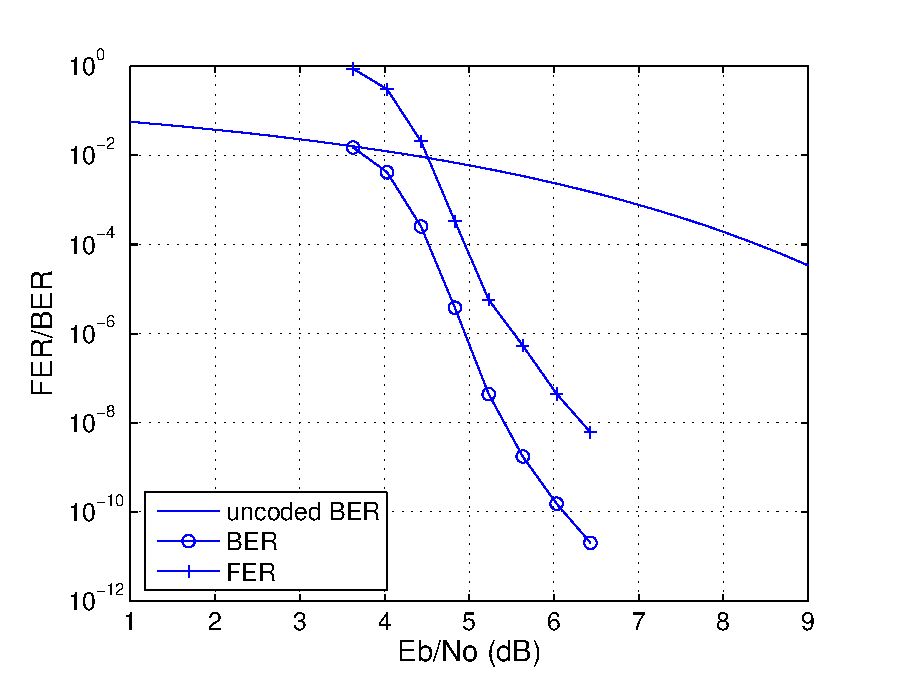
\includegraphics[keepaspectratio,width=3.0in,height=2.75in]{474_lara3.eps}
\caption{Experimental Results for $C_{47,4}$} \label{expif}
\end{figure}
%\newline \vspace{1.5in} \newline\vspace{0.0in}

%\vspace{1in}
%\vspace{4in}
\vspace{-0.00in}\section{Conclusion and Future Work}\label{conc}
%The conclusion goes here.



In this Chapter we presented a detailed analysis of the dominant
configurations in the error-floor regime of high rate array-based
LDPC codes. We provided an explicit description of the minimal
(fully) absorbing sets and showed the non-existence of certain
candidate configurations. We also enumerated minimal (fully)
absorbing sets and showed how their number scales with the
codeword length. Experiments on an emulation platform were
performed and were found to be in agreement with the theoretical
description of the dominant errors.
